
\documentclass{report}
% alternatives: scrartcl, article or report


%%%%% PACKAGES

% small tweaks and nicer typography
\usepackage{microtype}
\usepackage{hyperref}

% dealing with figures
\usepackage{subcaption}
\usepackage{wrapfig}

% basic math stuff
\usepackage{mathtools}
\usepackage{amssymb}
\usepackage{amsthm}
%\usepackage{tikz-cd}
\usepackage{cancel}
\usepackage{cases}
\usepackage{dsfont}

% tikz
\usepackage{tikz}
\usepackage{pgfplots}
\usetikzlibrary{positioning}
%\usetikzlibrary{patterns}
%\usetikzlibrary{babel}
\tikzset{>=stealth}
\usepackage{wrapfig}

% code
\usepackage{listings}
\usepackage{pythonhighlight}

%%%% Graphics %%%%%

%\graphicspath{{Plots/}}

%\newcommand{\tikzmark}[3][]{\tikz[remember picture,baseline] \node [anchor=base,#1](#2) {$#3$};}

%\usepackage{booktabs}
%\usepackage{bm}
%\usepackage{minted}

% for inkscape images
%\usepackage{pdftricks}
%\begin{psinputs}
%   \usepackage{pstricks}
%   \usepackage{multido}
%\end{psinputs}
%\usepackage[pdf]{pstricks}
%\usepackage{import}


\usepackage[backend=bibtex]{biblatex}
\addbibresource{mybib.bib}


%%%%% CONFIGURATION

% prevents automatic line breaks inside of equations
% since it looks bad
\binoppenalty = \maxdimen
\relpenalty   = \maxdimen

% theorem-like environments
\newcounter{everything}
\newtheorem{corollary}[everything]{Corollary}
\newtheorem{lemma}[everything]{Lemma}
\newtheorem{proposition}[everything]{Proposition}
\newtheorem{theorem}[everything]{Theorem}
\newtheorem*{claim}{Claim}
\newtheorem*{given}{Given}


%%%%% CUSTOM COMMANDS

% real numbers via \R
% complex numbers via \C
% general field via \K
\def\C{\mathbb{C}}
\def\R{\mathbb{R}}
\def\K{\mathbb{K}}
\def\Q{\mathbb{Q}}
\def\Z{\mathbb{Z}}
\def\N{\mathbb{N}}
\def\H{\mathbb{H}}
\def\e{\varepsilon}

\newcommand{\cA}{\mathcal{A}}
\newcommand{\cB}{\mathcal{B}}
\newcommand{\cC}{\mathcal{C}}
\newcommand{\cD}{\mathcal{D}}
\newcommand{\cE}{\mathcal{E}}
\newcommand{\cF}{\mathcal{F}}
\newcommand{\cG}{\mathcal{G}}
\newcommand{\cH}{\mathcal{H}}
\newcommand{\cI}{\mathcal{I}}
\newcommand{\cJ}{\mathcal{J}}
\newcommand{\cK}{\mathcal{K}}
\newcommand{\cL}{\mathcal{L}}
\newcommand{\cM}{\mathcal{M}}
\newcommand{\cN}{\mathcal{N}}
\newcommand{\cO}{\mathcal{O}}
\newcommand{\cP}{\mathcal{P}}
\newcommand{\cQ}{\mathcal{Q}}
\newcommand{\cR}{\mathcal{R}}
\newcommand{\cS}{\mathcal{S}}
\newcommand{\cT}{\mathcal{T}}
\newcommand{\cU}{\mathcal{U}}
\newcommand{\cV}{\mathcal{V}}
\newcommand{\cW}{\mathcal{W}}
\newcommand{\cX}{\mathcal{X}}
\newcommand{\cY}{\mathcal{Y}}
\newcommand{\cZ}{\mathcal{Z}}

\newcommand{\bA}{\mathbb{A}}
\newcommand{\bB}{\mathbb{B}}
\newcommand{\bC}{\mathbb{C}}
\newcommand{\bD}{\mathbb{D}}
\newcommand{\bE}{\mathbb{E}}
\newcommand{\bF}{\mathbb{F}}
\newcommand{\bG}{\mathbb{G}}
\newcommand{\bH}{\mathbb{H}}
\newcommand{\bI}{\mathbb{I}}
\newcommand{\bJ}{\mathbb{J}}
\newcommand{\bK}{\mathbb{K}}
\newcommand{\bL}{\mathbb{L}}
\newcommand{\bM}{\mathbb{M}}
\newcommand{\bN}{\mathbb{N}}
\newcommand{\bO}{\mathbb{O}}
\newcommand{\bP}{\mathbb{P}}
\newcommand{\bQ}{\mathbb{Q}}
\newcommand{\bR}{\mathbb{R}}
\newcommand{\bS}{\mathbb{S}}
\newcommand{\bT}{\mathbb{T}}
\newcommand{\bU}{\mathbb{U}}
\newcommand{\bV}{\mathbb{V}}
\newcommand{\bW}{\mathbb{W}}
\newcommand{\bX}{\mathbb{X}}
\newcommand{\bY}{\mathbb{Y}}
\newcommand{\bZ}{\mathbb{Z}}

\newcommand{\dif}[1]{\,\mathrm{d} #1}
%\newcommand{\norm}[1]{\lVert #1 \rVert}
%\newcommand{\abs}[1]{\left| #1 \right|}
\newcommand{\bnorm}[1]{\left\lVert #1\right\rVert}
\newcommand{\vii}[2]{\ensuremath{\begin{bmatrix}#1 \\ #2 \end{bmatrix}}}
\newcommand{\mii}[4]{\ensuremath{\begin{bmatrix}#1&#2 \\ #3&#4 \end{bmatrix}}}
\newcommand{\mc}[1]{\mathcal{#1}}

\newcommand{\one}{\mathds{1}}
\newcommand{\bigO}{\mathcal{O}}


%%%%%%%%%%    Math operators    %%%%%%%%%%%%%%%%%%%%%%%%%%%

\DeclareMathOperator{\Id}{Id}             % identity morphism
% \DeclareMathOperator{\ker}{ker}           % kernel
\DeclareMathOperator{\rg}{rg}             % image
\DeclareMathOperator{\defekt}{def}             % defect
\DeclareMathOperator{\im}{im}             % image
\DeclareMathOperator{\Hom}{Hom}           % homomorphisms
\DeclareMathOperator{\End}{End}           % endomorphisms
\DeclareMathOperator{\Span}{Span}         % linear span
\DeclareMathOperator{\grad}{\nabla}         % gradient
\DeclareMathOperator{\diam}{diam}         % gradient
\DeclareMathOperator{\Tr}{Tr}       	  % trace
\DeclareMathOperator{\diver}{Div}			% divergence
\DeclareMathOperator{\supp}{supp}			% support
\DeclareMathOperator{\dist}{dist}			% distance
\DeclareMathOperator{\inter}{int}			% interiour
\DeclareMathOperator{\epi}{epi}			% epigraph
\DeclareMathOperator{\hyp}{hyp}			% hypograph
\DeclareMathOperator{\Lip}{Lip}			% lipschitz konstant
\DeclareMathOperator{\graph}{graph}			% graph
\DeclareMathOperator{\sgn}{sgn}			% sign
\DeclareMathOperator{\BMO}{BMO}			% BMO
\DeclareMathOperator{\mean}{mean}			% BMO
%\DeclareMathOperator{\B}{B}			% BMO

% inner product (scalar product) via \inner{v, w}
% norm via \norm{x}
% absolute value via \abs{x}
% use the star-version for automatic scaling
\DeclarePairedDelimiter{\abs}{\lvert}{\rvert}
\DeclarePairedDelimiter{\inner}{\langle}{\rangle}
\DeclarePairedDelimiter{\norm}{\lVert}{\rVert}

% \vect{ x // y // z } for a column vector with entries x, y, z
% similarly for larger vectors
% in this code:  1 = number of arguments
%               #1 = first argument
\newcommand{\vect}[1]{\begin{bmatrix} #1 \end{bmatrix}}
\newcommand{\commentops}[2]{\stackrel{\mathclap{#1}}{#2}}


% \conj{z} for complex conjugation
\newcommand{\conj}{\overline}

%counter of current constant number:    
\newcounter{constant} 
%defines a new constant, but does not typeset anything:
\newcommand{\newconstant}[1]{\refstepcounter{constant}\label{#1}} 
%typesets named constant:
\newcommand{\useconstant}[1]{c_{\ref{#1}}}

%%%%%%% GENERAL STYLE %%%%%%%%%%%%%%%%%%

%\setcounter{tocdepth}{3}


%%%%% TITLE PAGE

%\subject{Simulation Tools, VT23}
\title{ Project Reports \\[1ex]
	  \large NUMN26 / FMNN05, Simulation Tools}
\author{Salvador Castagnino, Theo Koppenhöfer}
\date{Lund \\[1ex] \today}


%%%%% The content starts here %%%%%%%%%%%%%


\begin{document}

\maketitle

\chapter*{Project 1}

\section*{Introduction}

In the following report we will discuss our implementation of the projects to the course NUMN26 / FMNN05, Simulation Tools. During the project we try out solvers from the \pyth{Assimulo} package which wraps the SUNDIALS ODE solvers and in project 3 briefly the \pyth{dune} package for discretising PDEs. In project 1 we will use a variant of the pendulum as a toy problem to test various explicit solvers of Assimulo. In project 2 we will then use a mechanical model of a seven body mechanism in various formulations as a benchmark to test Assimulo's implicit solvers. In project 3 we then test an implementation of the explicit Newmark method on the pendulum and an implementation of the HHT-$\alpha$ and the implicit Newmark solvers on a discretised PDE given by an elastic beam.
This report and the code belonging to it can be found online under \cite{Repository}.

\subsection*{The Benchmark}


\begin{wrapfigure}{r}{0.43\textwidth}
\centering
\input{../Drawings/pendulum.pdf_tex}
\caption{The pendulum}
\label{dr:Pendulum}
\vspace*{-1cm}
\end{wrapfigure}

In the following we use the model of a pendulum attached to a rod which is elastic in the radial direction. The situation is depicted in figure \ref{dr:Pendulum}.
This problem leads to the formulation as an ODE
\begin{align*}
	\vect{y_1 \\ y_2 \\ y_3 \\ y_4}' = \vect{y_3 \\ y_4 \\ -y_1\lambda(y_1,y_2) \\ -y_2\lambda(y_1,y_2)-1}
\end{align*}
with
\begin{align*}
	\lambda(y_1,y_2)=k\frac{\norm{(y_1,y_2)}-1}{\norm{(y_1,y_2)}}\,.
\end{align*}
The plot of a numerical solution to this problem for $k=1$ can be seen in figures \ref{pl:StateTime1}, \ref{pl:PhasePortrait1} and \ref{pl:PolarPlot1}.

\begin{figure}[h]
\centering
\begin{minipage}[b]{0.45\textwidth}
\centering
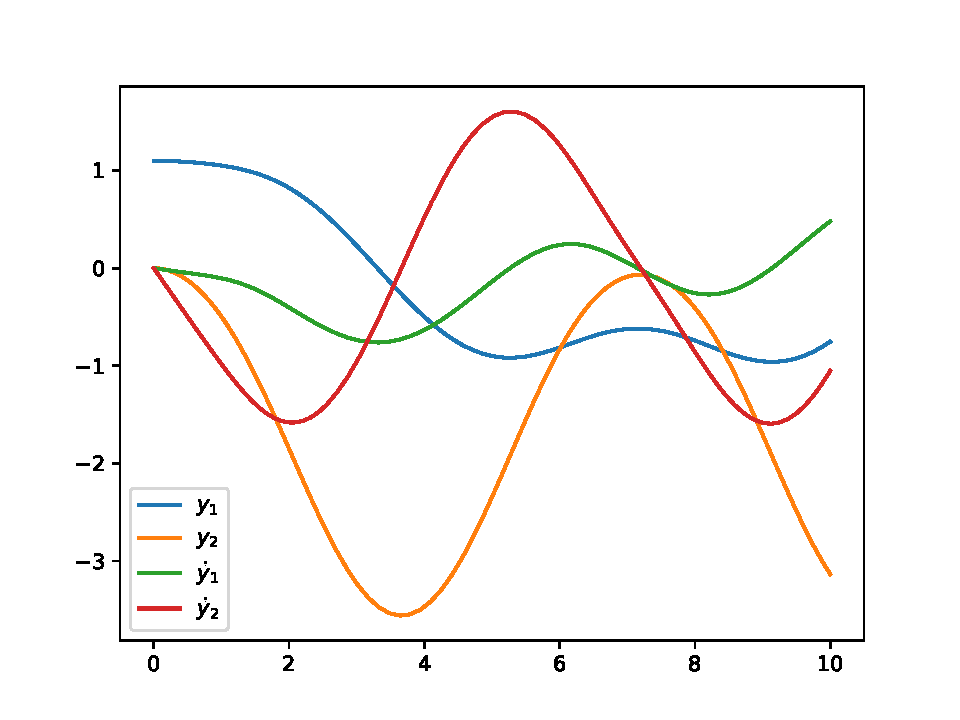
\includegraphics[width=\textwidth]{../Plots/Task4/Figure_1}
\caption{State in dependence of time.}
\label{pl:StateTime1}
\end{minipage}
\hfill
\begin{minipage}[b]{0.45\textwidth}
\centering
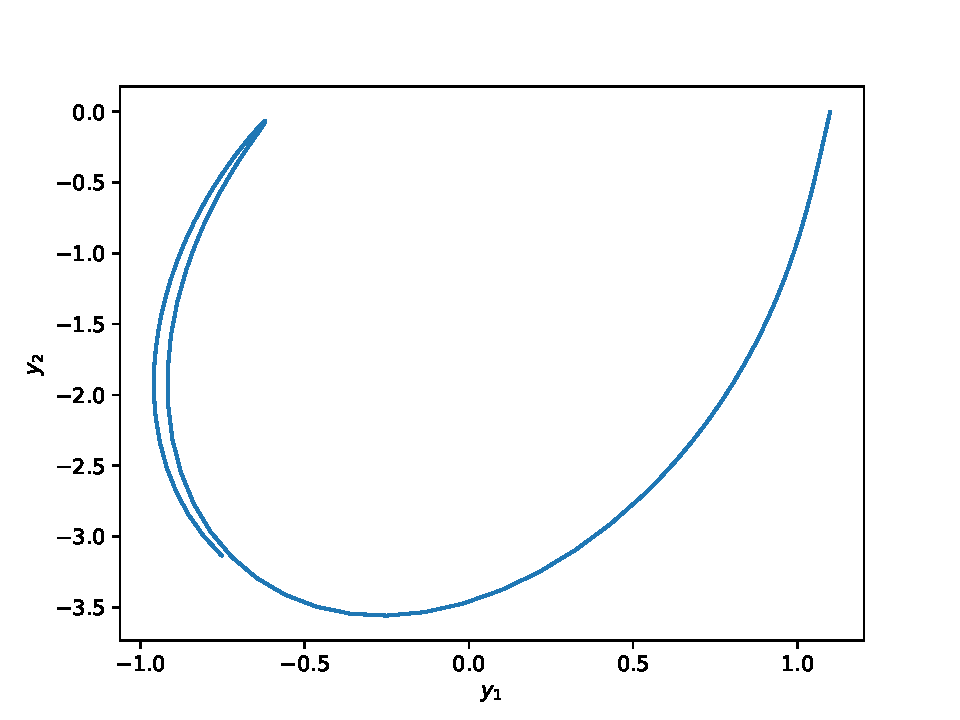
\includegraphics[width=\textwidth]{../Plots/Task4/Figure_2}
\caption{Path traced out by pendulum.}
\label{pl:PhasePortrait1}
\end{minipage}
\end{figure}

We can calculate the potential, kinetic and approximate elastic energies with the formulas
\begin{align*}
	E_{\text{pot}}=1+y_2
	\qquad E_{\text{kin}}=\frac{\norm{(y_3,y_4)}^2}{2}
	\qquad E_{\text{elast}}=k\frac{(\norm{(y_1,y_2)}-1)^2}{2}\,.
\end{align*}
Adding these up we get the approximate total energy
\begin{align*}
	E_{\text{tot}}=E_{\text{pot}}+E_{\text{kin}}+E_{\text{elast}}\,.
\end{align*}
We expect the approximate total energy to be almost constant which indeed can be seen in figure \ref{pl:EnergyPlot1} for that previously calculated numerical solution.
Because of this property we can use the variance of the approximate total energy as an index to measure the stability of a solver. 
In the ideal world this index almost vanishes.

\begin{figure}[h]
\centering
\begin{minipage}[b]{0.45\textwidth}
\centering
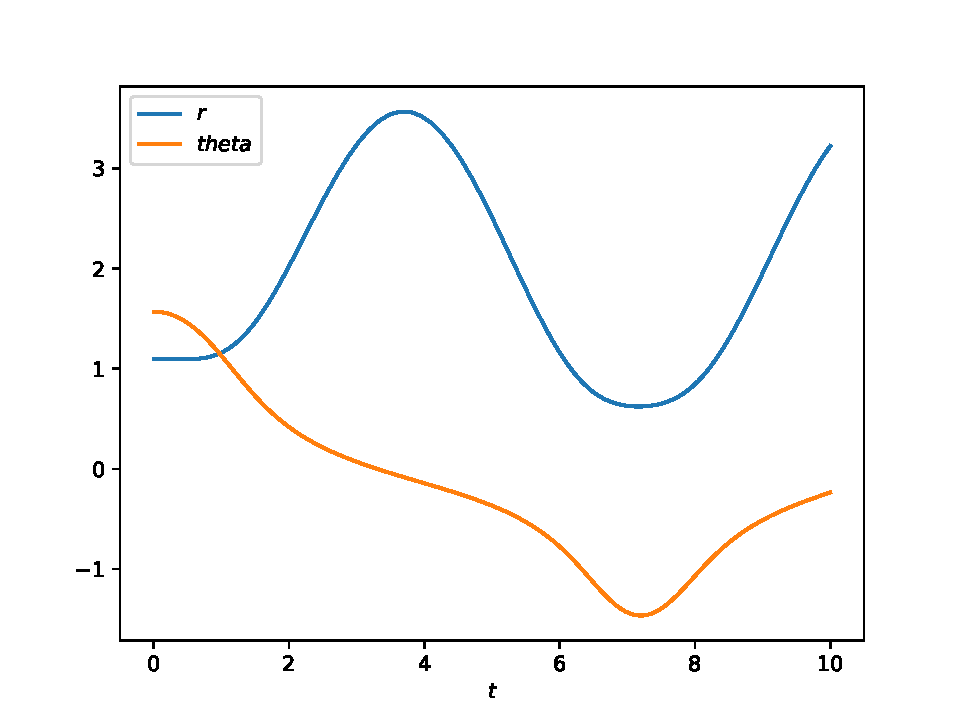
\includegraphics[width=\textwidth]{../Plots/Task4/Figure_0}
\caption{Polar coordinates.}
\label{pl:PolarPlot1}
\end{minipage}
\hfill
\begin{minipage}[b]{0.45\textwidth}
\centering
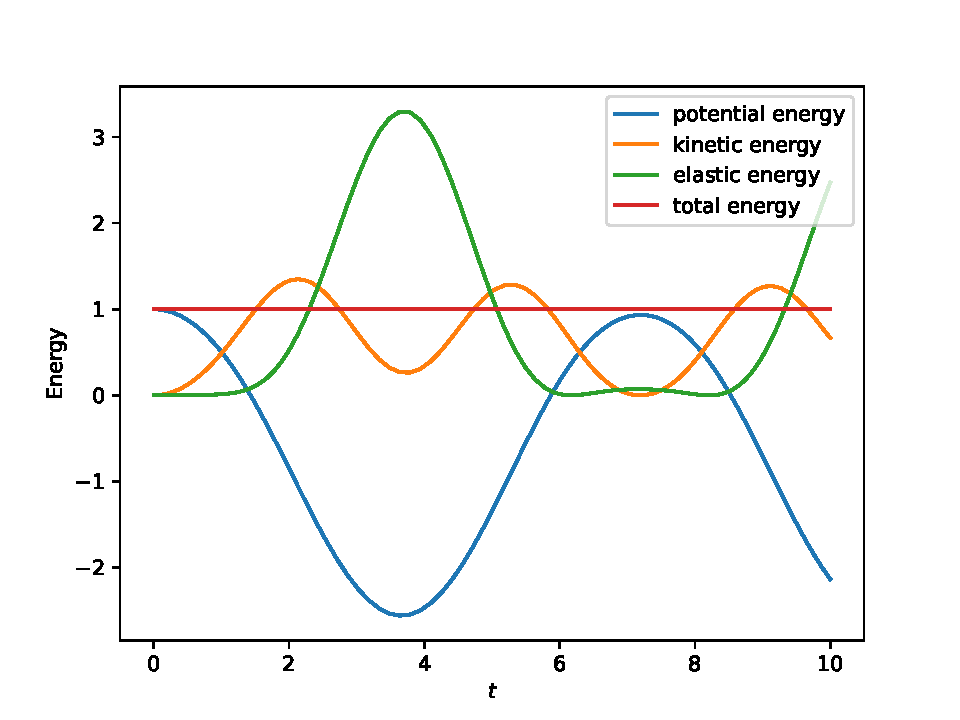
\includegraphics[width=\textwidth]{../Plots/Task4/Figure_3}
\caption{Energy plot}
\label{pl:EnergyPlot1}
\end{minipage}
\end{figure}

\section*{Testing Explicit Methods}

With increasing $k$ the elastic pendulum problem behaves increasingly stiff. As explicit methods have a relatively small stability region when compared with the left-half plane this means the step size $h$ has to be reduced with increasing $k$ for the numerical solution to remain bounded.

%\begin{figure}[h]
%\centering
%\begin{minipage}[b]{0.45\textwidth}
%\centering
%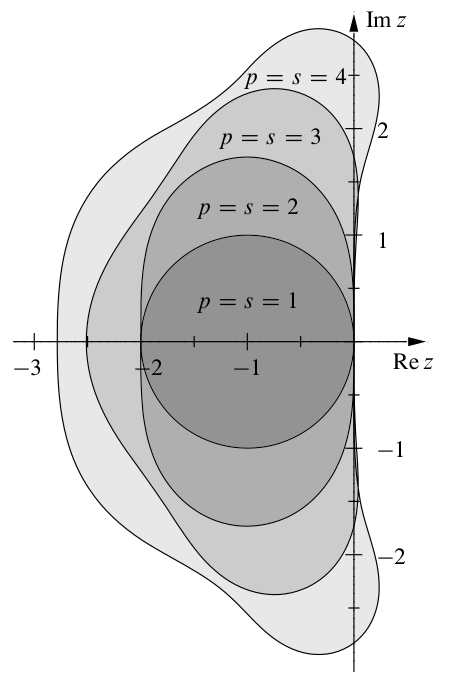
\includegraphics[width=\textwidth]{../Drawings/Runge_Kutter_stability_regions}
%\caption{Stability regions of the Runge-Kutta-methods, taken from \cite{Stab_RK}[p.238]}
%\end{minipage}
%\end{figure}

The problem was simulated using Explicit Euler and RK4.
All the experiments in this section are simulated on the domain $[0,20]$ and have initial the initial value $$y_0 = \vect{1.1 \\ 0 \\ 0 \\ 0}\,.$$
The graphs are presented in polar coordinates where $r$ refers to the length of the spring and $\theta$ refers to the angle between the pendulum and the vertical axis.

It can be observed that for the fixed step size $h=0.01$ Explicit Euler (figure \ref{exp_euler_k=50_h=0.01_c}) already shows instability for values of $k=50$ while RK4 (figure \ref{rk4_h=0.01_k=3000_c}) remains stable for values up to $k=3000$.

\begin{figure}[h]
\centering
\begin{minipage}[t]{0.45\textwidth}
\centering
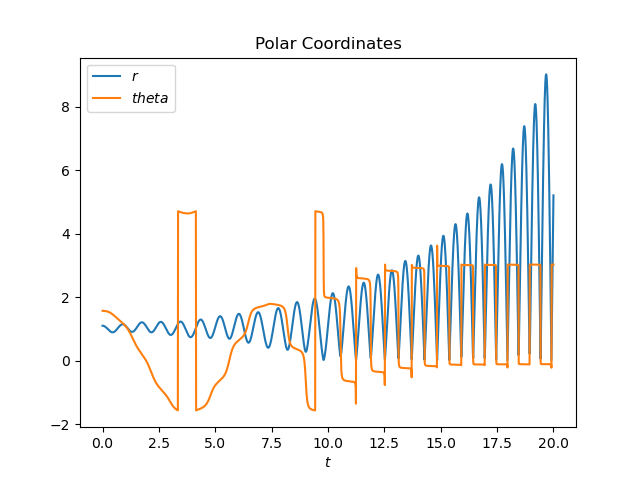
\includegraphics[width=\textwidth]{../Plots/ExpEuler/exp_euler_k=50_h=0.01_c}
\caption{Explicit Euler with parameters $h=0.01$ and $k=50$.}
\label{exp_euler_k=50_h=0.01_c}
\end{minipage}
\hfill
\begin{minipage}[t]{0.45\textwidth}
\centering
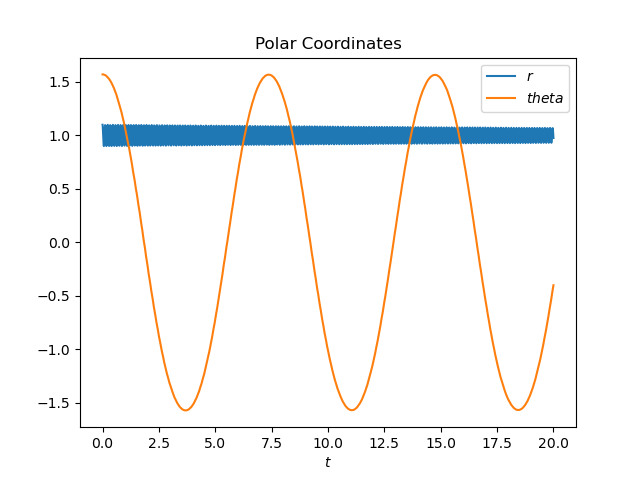
\includegraphics[width=\textwidth]{../Plots/RK4/rk4_h=0.01_k=3000_c}
\caption{RK4 with parameters $h=0.01$ and $k=3000$.}
\label{rk4_h=0.01_k=3000_c}
\end{minipage}
\end{figure}

\begin{wrapfigure}{r}{0.50\textwidth}
\vspace*{-0.8cm}
\raggedleft
\begin{minipage}[b]{0.45\textwidth}
\centering
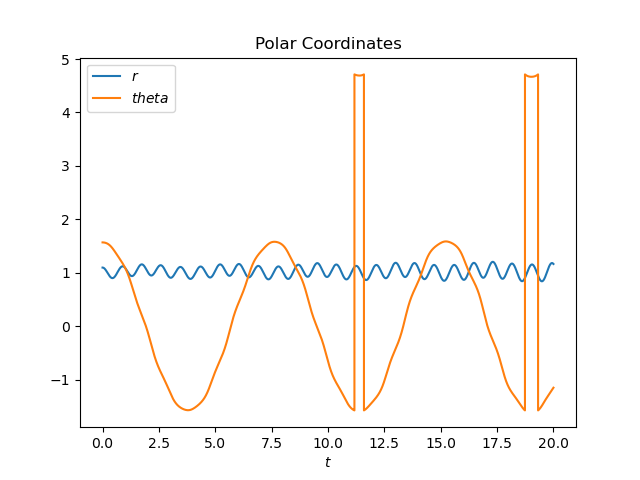
\includegraphics[width=\textwidth]{../Plots/ExpEuler/exp_euler_k=50_h=0.001_c}
\caption{Explicit Euler with parameters $h=0.001$ and $k=50$.}
\label{exp_euler_k=50_h=0.001_c_2}
\end{minipage}
\end{wrapfigure}
	
By keeping the value of $k$ constant and reducing the step size by an order of magnitude with Explicit Euler (c.f.\ figure \ref{exp_euler_k=50_h=0.001_c_2}) we see how the instability is attenuated and it thus presents a similar amplitude over time.
It takes a much larger step size and spring constant for RK4 to become unstable as can be seen in figure \ref{rk4_h=0.1_k=975_c}. Furthermore its growth is much more rapid than Explicit Euler’s when unstable and occurs without oscillating.


\begin{figure}[h]
\centering
\begin{minipage}[b]{0.45\textwidth}
\centering
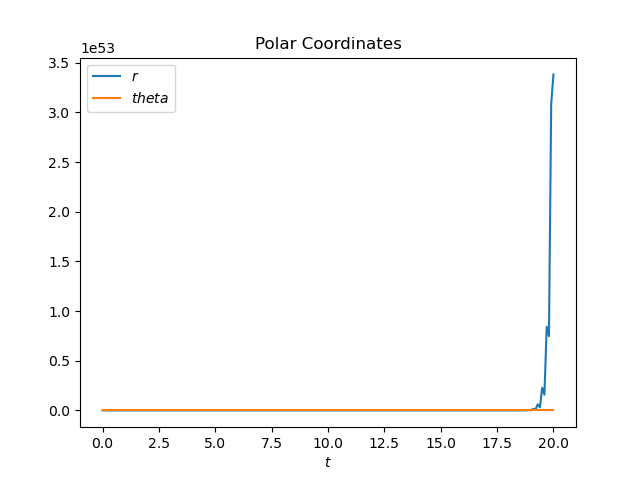
\includegraphics[width=\textwidth]{../Plots/RK4/rk4_h=0.1_k=975_c}
\caption{RK4 with parameters $h=0.1$ and $k=975$.}
\label{rk4_h=0.1_k=975_c}
\end{minipage}
\hfill
\begin{minipage}[b]{0.45\textwidth}
\centering
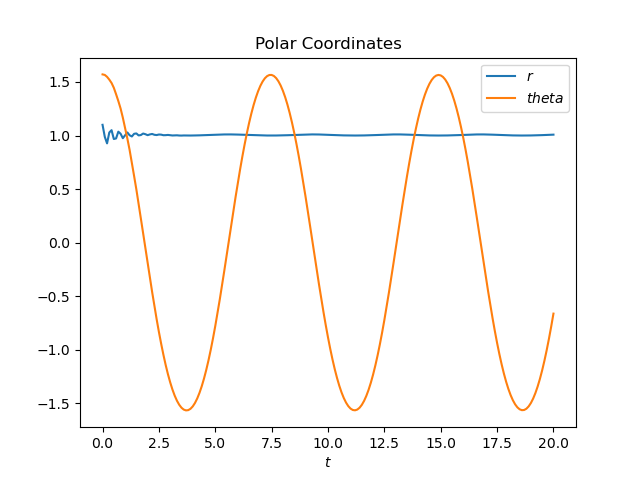
\includegraphics[width=\textwidth]{../Plots/RK4/rk4_h=0.1_k=300_c}
\caption{RK4 with parameters $h=0.1$ and $k=300$.}
\label{rk4_h=0.1_k=300_c}
\end{minipage}
\end{figure}

It is interesting to observe that the oscillation of the spring is rapidly damped with RK4 (figure \ref{rk4_h=0.1_k=300_c}), a behavior similar to that presented by implicit methods.
This behavior was not observed in the other explicit methods.


\section*{Testing Implicit Methods}

In contrast to explicit methods for linear problems implicit methods have an extensive stability region. Hence their stability does not depend on the value of the step $k$.
The problem was simulated using Implicit Euler, BDF2 with Fixed Point as corrector and BDFk with Newton as corrector for $k$ between $1$ and $4$. Unless otherwise stated the following experiments have $[0,20]$ as domain and initial value $$y_0 = \vect{1.1 \\ 0 \\ 0 \\ 0}\,.$$
It is interesting to see how the oscillation of the spring decays for implicit methods. This decay can be attenuated by reducing the step size or accelerated by increasing the value of the spring constant.

\begin{figure}[h]
\centering
\begin{minipage}[b]{0.45\textwidth}
\centering
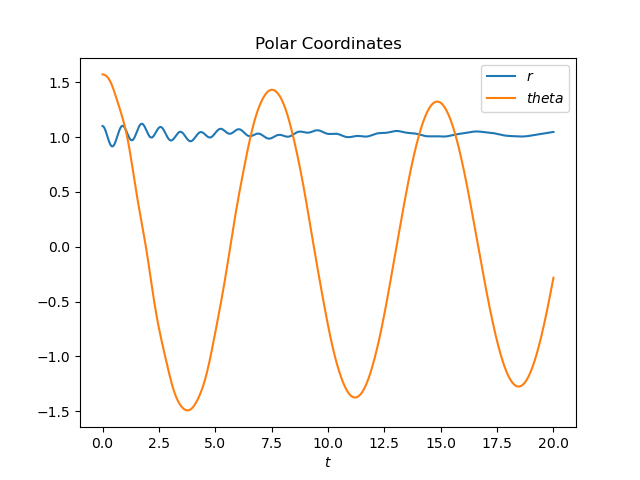
\includegraphics[width=\textwidth]{../Plots/ImpEuler/imp_euler_h=0.01_k=50_c}
\caption{Implicit Euler with parameters $h=0.01$ and $k=50$.}
\label{imp_euler_h=0.01_k=50_c}
\end{minipage}
\end{figure}

\begin{figure}[h]
\centering
\begin{minipage}[b]{0.45\textwidth}
\centering
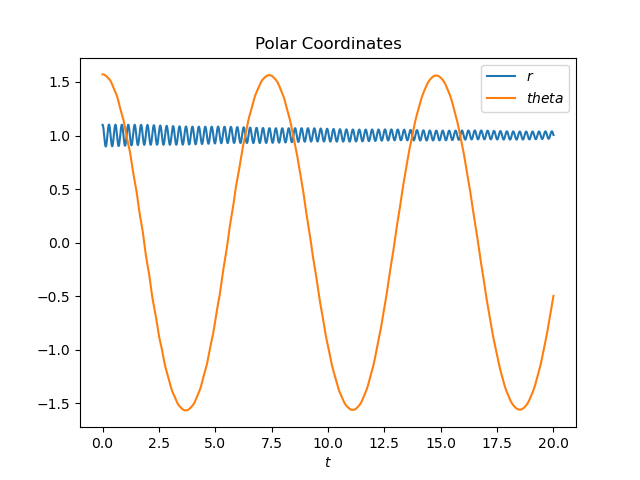
\includegraphics[width=\textwidth]{../Plots/BDF2/bdf2_h=0.01_k=500_c}
\caption{BDF2 with parameters $h=0.001$ and $k=500$.}
\label{exp_euler_k=50_h=0.001_c}
\end{minipage}
\hfill
\begin{minipage}[b]{0.45\textwidth}
\centering
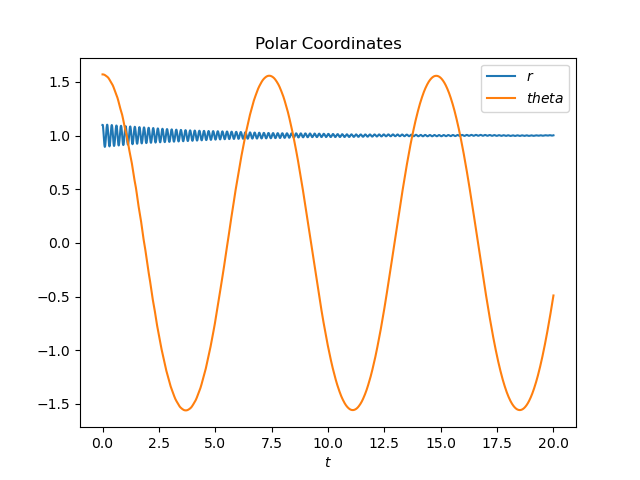
\includegraphics[width=\textwidth]{../Plots/BDF2/bdf2_h=0.01_k=1000_c}
\caption{BDF2 with parameters $h=0.01$ and $k=1000$.}
\label{bdf2_h=00.1_k=1000_c}
\end{minipage}
\end{figure}

The BDFk method with Newton presents a decay in the spring oscillation as the other methods do.
However, it also shows decay of the pendulum oscillation which cannot be observed in the other implicit methods.
To better observe this decay (figure \ref{bdf2_h=0.01_h=100_tf=100} and figure \ref{bdf4_h=0.01_h=100_tf=100.png}) the domain is increased to $[0, 100]$.

\begin{figure}[h]
\centering
\begin{minipage}[b]{0.45\textwidth}
\centering
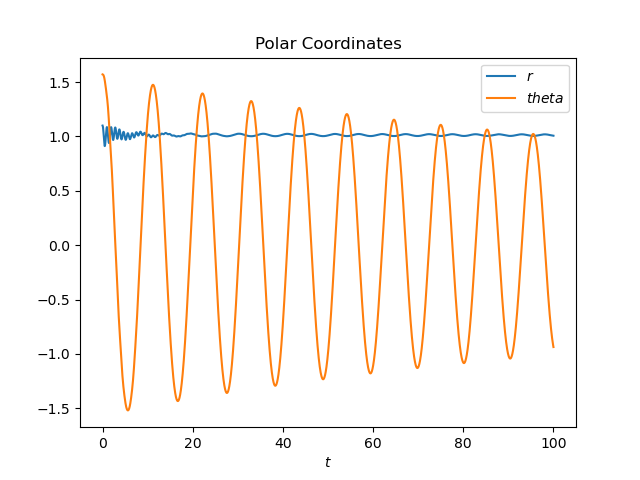
\includegraphics[width=\textwidth]{../Plots/BDFk/bdf2_h=0.01_h=100_tf=100}
\caption{BDF2-Newton $h=0.01$ $k=100$}
\label{bdf2_h=0.01_h=100_tf=100}
\end{minipage}
\hfill
\begin{minipage}[b]{0.45\textwidth}
\centering
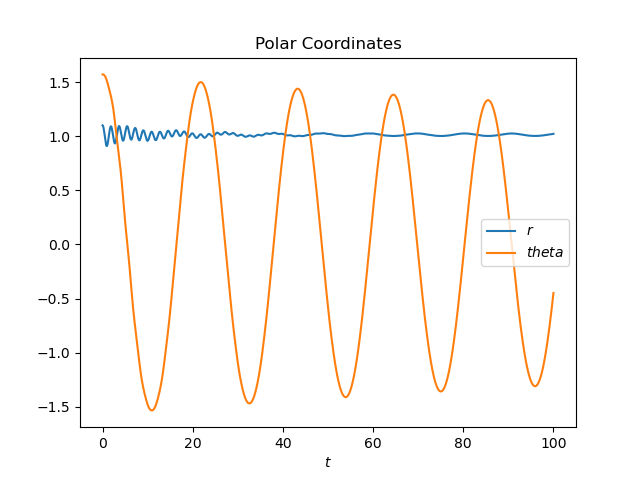
\includegraphics[width=\textwidth]{../Plots/BDFk/bdf4_h=0.01_h=100_tf=100}
\caption{BDF4-Newton $h=0.01$ $k=100$}
\label{bdf4_h=0.01_h=100_tf=100.png}
\end{minipage}
\end{figure}

It is interesting to see how the relation between the speed of decay of the spring oscillation in inversely related to the size of the stability region of the methods tested.


\newpage
\newpage


\section*{Testing CVODE}
\subsection*{A first test series}

In the first specific test of CVODE we solve our toy problem for increasing $k$. Here we switch between the BDF and Adam-Moulton's discretisation method. We also vary the \pyth{maxorder} parameter for both methods.
A higher $k$ causes a stiffer problem. As a stiff problem requires smaller steps the number of steps \pyth{nsteps} increases as $k$ increases which  can be seen in figure \ref{pl:nsteps1}. As the number of function evaluations per step size, \pyth{nfcns/nsteps}, hovers slightly above 1 for all methods (c.f.\ figure \ref{pl:nfcns_nsteps1}) the number of function evaluations increase proportionally to \pyth{nsteps} with $k$ as can be seen in figure \ref{pl:nfcns1}. There is however a difference in how many steps each method needs. The BDF-method requires in general more steps than the Adams-Moulton method. In general the number of steps increases as \pyth{maxord} is reduced. 

\begin{figure}[h]
\centering
\begin{minipage}[b]{0.45\textwidth}
\centering
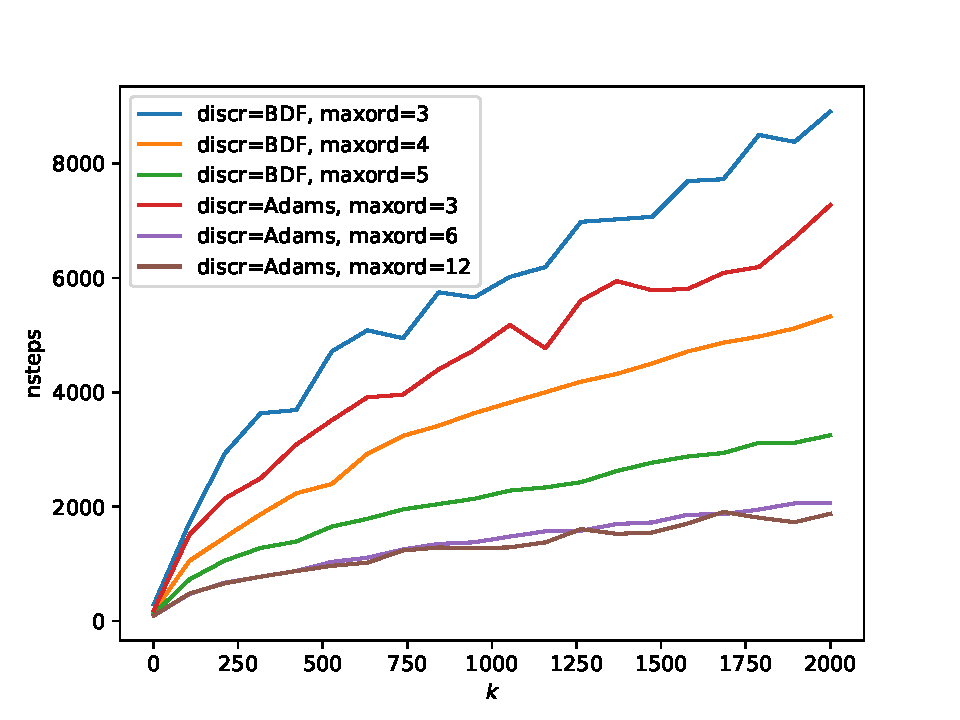
\includegraphics[width=\textwidth]{../Plots/Task4/Figure_200}
\caption{\pyth{nsteps} in relation to the parameter $k$.}
\label{pl:nsteps1}
\end{minipage}
\hfill
\begin{minipage}[b]{0.45\textwidth}
\centering
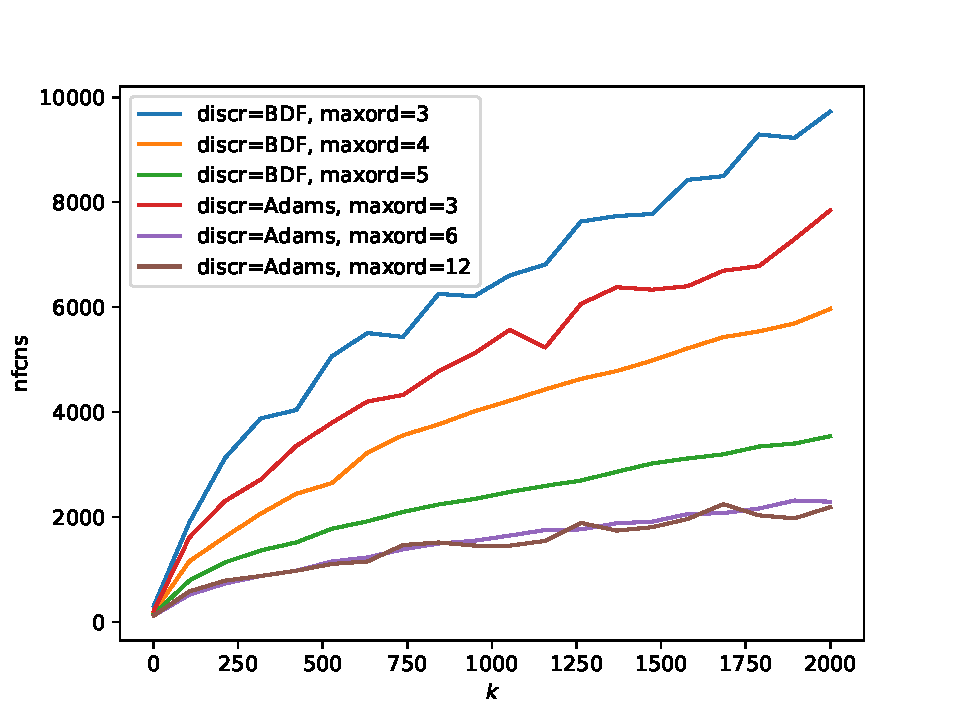
\includegraphics[width=\textwidth]{../Plots/Task4/Figure_201}
\caption{\pyth{nfuncs} in relation to the parameter $k$.}
\label{pl:nfcns1}
\end{minipage}
\end{figure}

\begin{figure}[h]
\centering
\begin{minipage}[b]{0.45\textwidth}
\centering
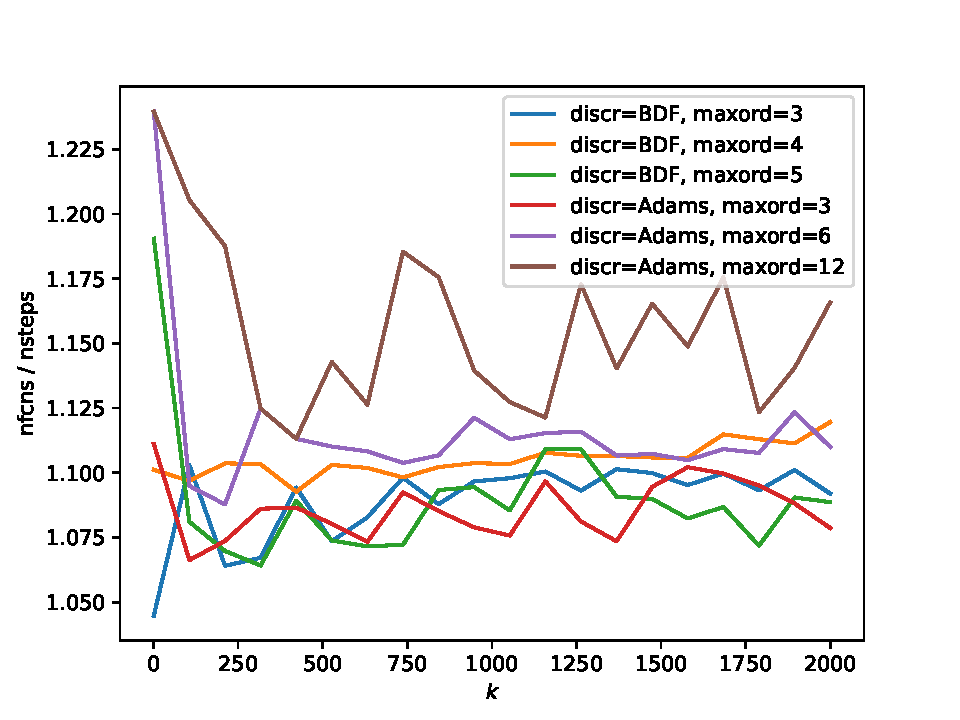
\includegraphics[width=\textwidth]{../Plots/Task4/Figure_210}
\caption{\pyth{nfcns/nsteps} in relation to the parameter $k$.}
\label{pl:nfcns_nsteps1}
\end{minipage}
\hfill
\begin{minipage}[b]{0.45\textwidth}
\centering
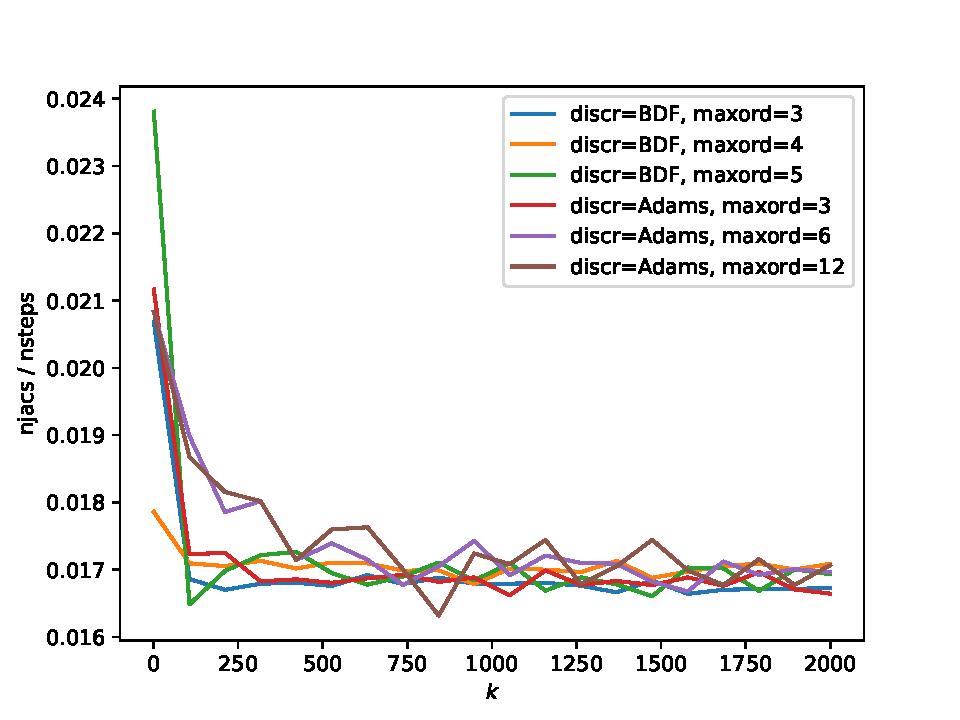
\includegraphics[width=\textwidth]{../Plots/Task4/Figure_211}
\caption{\pyth{njacs/nsteps} in relation to the parameter $k$.}
\label{pl:njacs_nsteps1}
\end{minipage}
\end{figure}

One sees in figure \ref{pl:njacs_nsteps1} that the number of Jacobian evaluations stays roughly constant and happens roughly every 5'th step. The number \pyth{nerrfails/steps} stays roughly constant in dependence of $k$ though in general it decreases with decreasing \pyth{maxord}. This makes sense because a lower \pyth{maxord} means there are fewer possibilities for the method order and hence fewer changes of order. In figure \ref{pl:stability1} we see a difference in how much the methods obey the principles of energy conservation. One can see that for growing $k$ the result diverge away from physical reality. Once again the methods with higher \pyth{maxord} do better with the exception of the BDF method where for some reason a \pyth{maxord} of 4 performs best.

\begin{figure}[h]
\centering
\begin{minipage}[b]{0.45\textwidth}
\centering
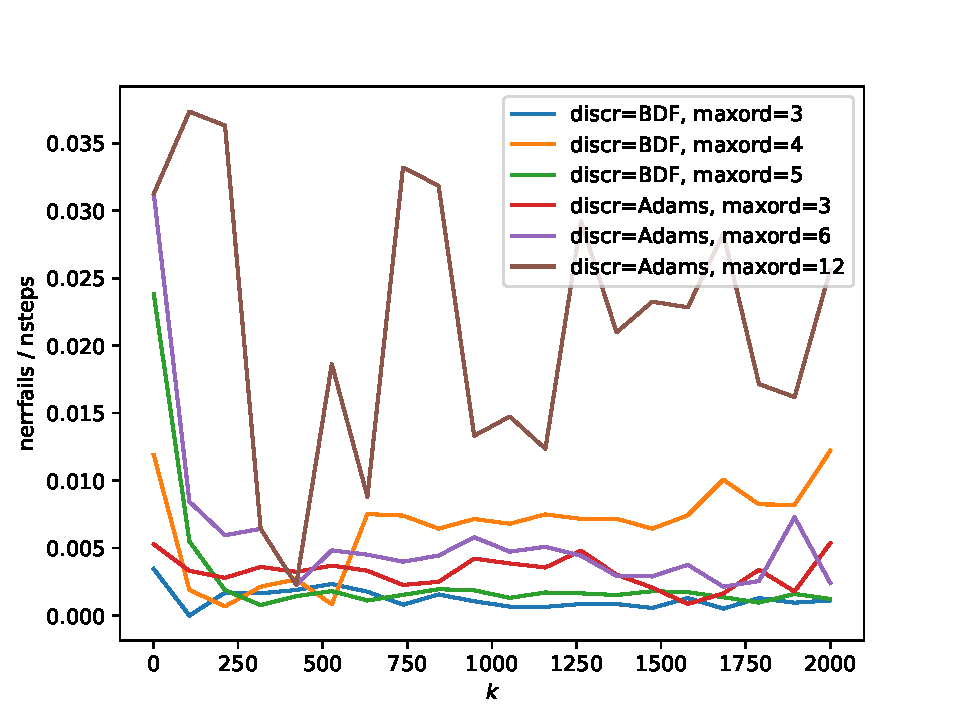
\includegraphics[width=\textwidth]{../Plots/Task4/Figure_212}
\caption{\pyth{nerrfails/nsteps} in relation to the parameter $k$.}
\label{pl:nerrfails_nsteps1}
\end{minipage}
\hfill
\begin{minipage}[b]{0.45\textwidth}
\centering
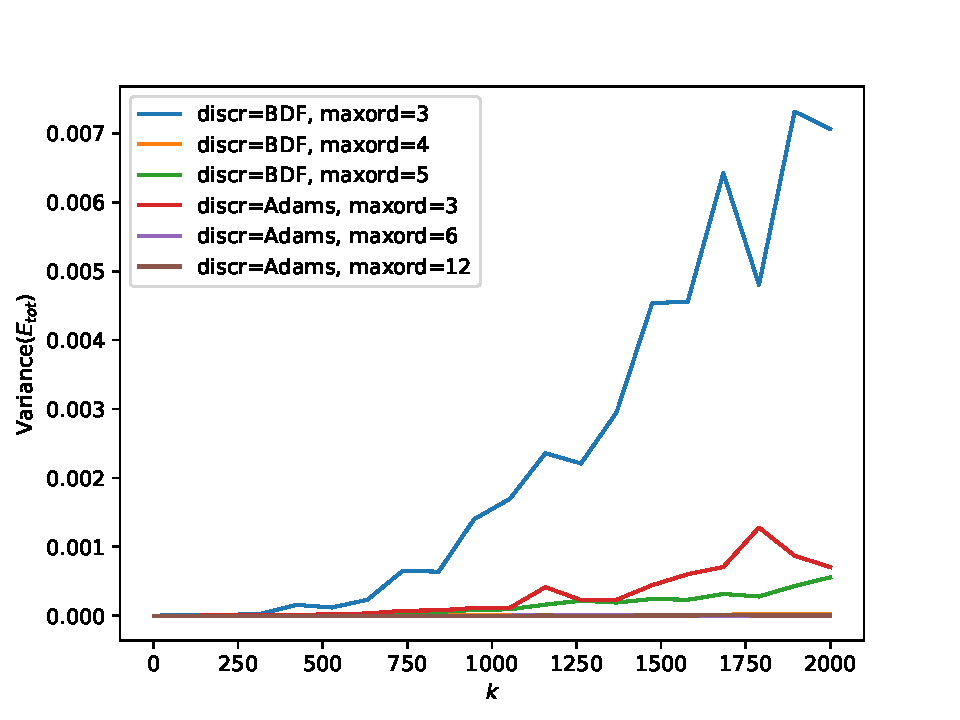
\includegraphics[width=\textwidth]{../Plots/Task4/Figure_204}
\caption{Variance of the energy in relation to the parameter $k$.}
\label{pl:stability1}
\end{minipage}
\end{figure}

This test confirms once again that stiffer problems need more function evaluations in CVODE.
Also, the Adams-Moulton-method seems to perform better on this problem.
This experiment also highlights that a lower \pyth{maxord} parameter tends to be more computationally expensive though it reduces the number of error test failures \pyth{nerrfails}.

\subsection*{Testing the parameter rtol}

\begin{wrapfigure}{r}{0.45\textwidth}
\centering
\begin{minipage}[t]{0.45\textwidth}
\centering
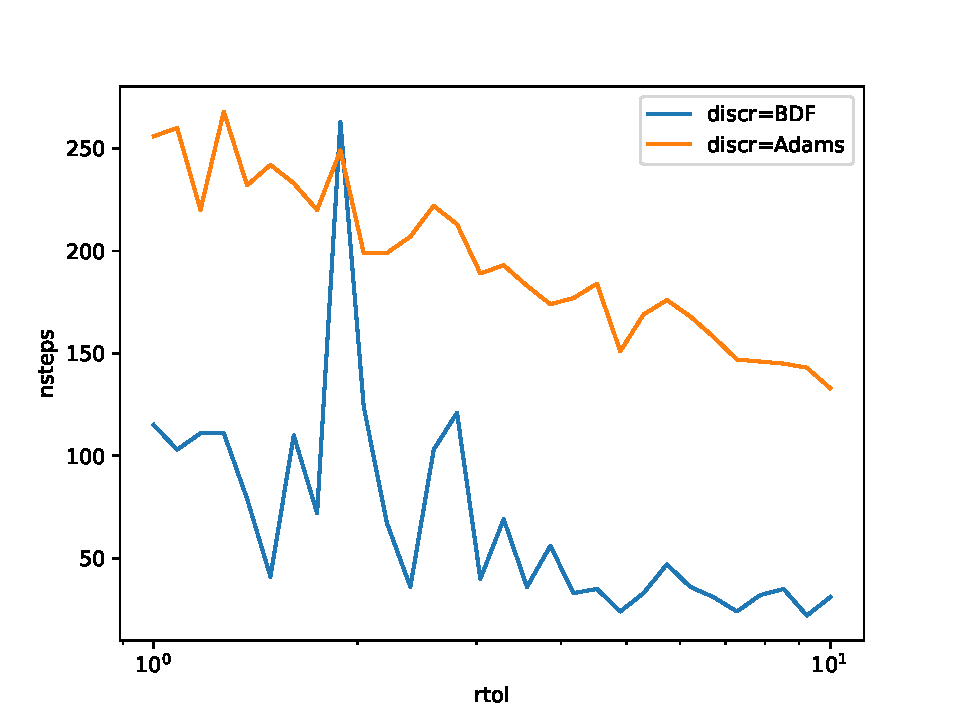
\includegraphics[width=\textwidth]{../Plots/Task4/Figure_300}
\caption{\pyth{nsteps} in relation to the parameter \pyth{rtol}.}
\label{pl:nsteps2}
\end{minipage}
\end{wrapfigure}

We now test the influence of the parameter \pyth{rtol} on the methods BDF and Adams-Moulton. For this we set $k=10^3$ and keep all other parameters on their default values. The results can be seen in figures \ref{pl:nsteps2} to \ref{pl:stability2}. We note that as \pyth{rtol} increases the number of steps decreases (c.f.\ figure \ref{pl:nsteps2}).The general tendency is that the number of Jacobian evaluations per step (figure \ref{pl:njacs_nsteps2}) and the number of error test failures per step (figure \ref{pl:nerrfails_nsteps2}) increases with \pyth{rtol}. We see in \ref{pl:stability2} that for large \pyth{rtol} the simulation with Adams-Moulton defies physics which indicates instability.

\begin{figure}[h]
\centering
\begin{minipage}[b]{0.45\textwidth}
\centering
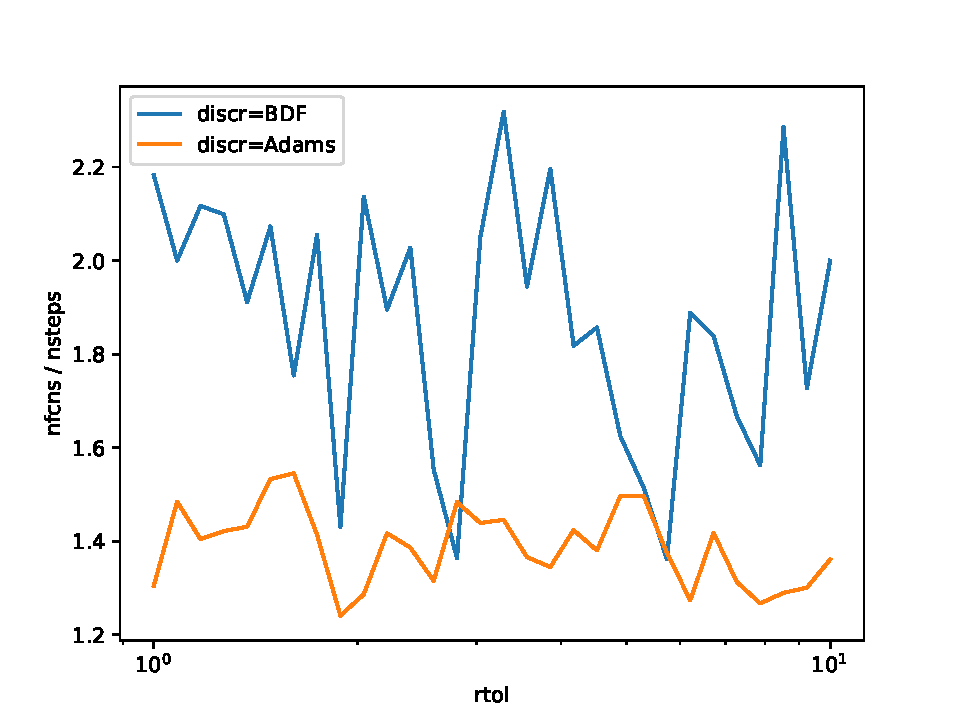
\includegraphics[width=\textwidth]{../Plots/Task4/Figure_310}
\caption{\pyth{nfcns/nsteps} in relation to the parameter \pyth{rtol}.}
\label{pl:nfcns_nsteps2}
\end{minipage}
\hfill
\begin{minipage}[b]{0.45\textwidth}
\centering
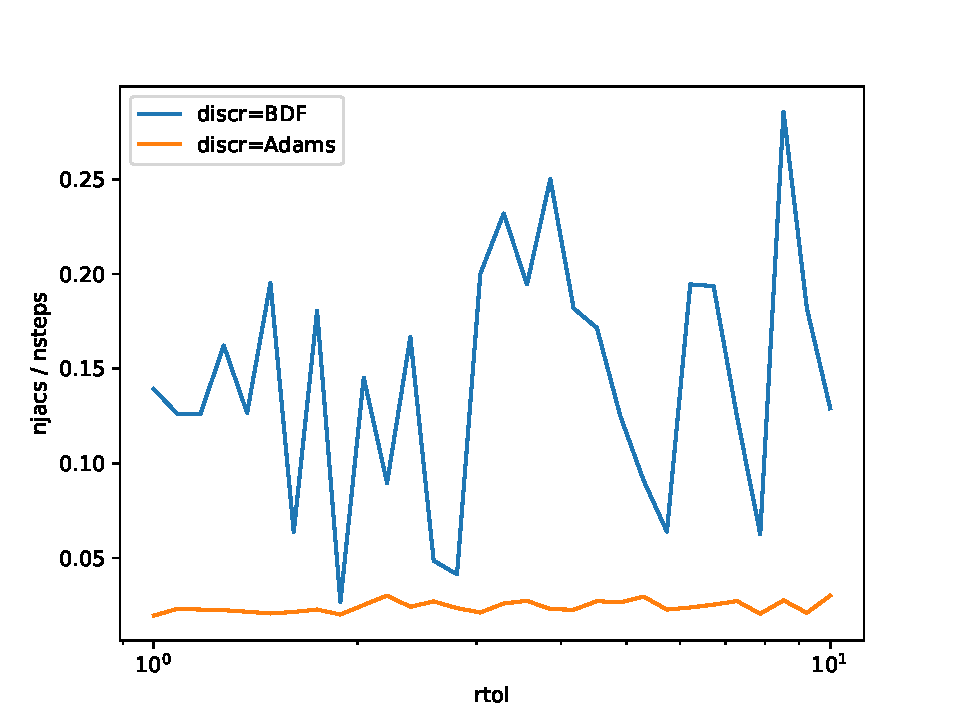
\includegraphics[width=\textwidth]{../Plots/Task4/Figure_311}
\caption{\pyth{njacs/nsteps} in relation to the parameter \pyth{rtol}.}
\label{pl:njacs_nsteps2}
\end{minipage}
\end{figure}


\begin{figure}[h]
\centering
\begin{minipage}[b]{0.45\textwidth}
\centering
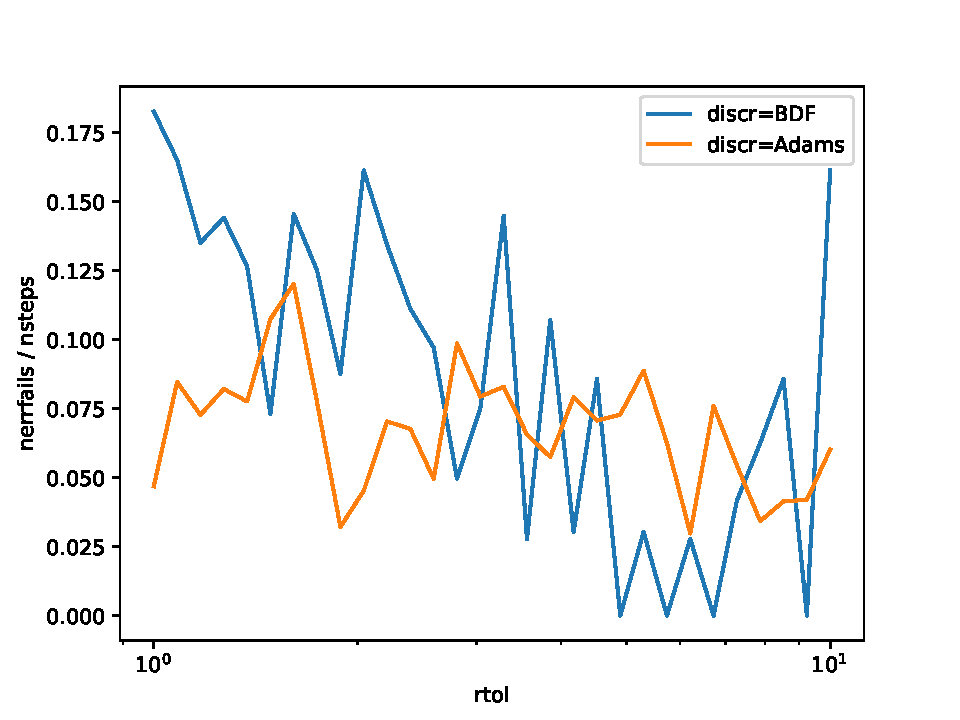
\includegraphics[width=\textwidth]{../Plots/Task4/Figure_312}
\caption{\pyth{nerrfails/nsteps} in relation to the parameter \pyth{rtol}.}
\label{pl:nerrfails_nsteps2}
\end{minipage}
\hfill
\begin{minipage}[b]{0.45\textwidth}
\centering
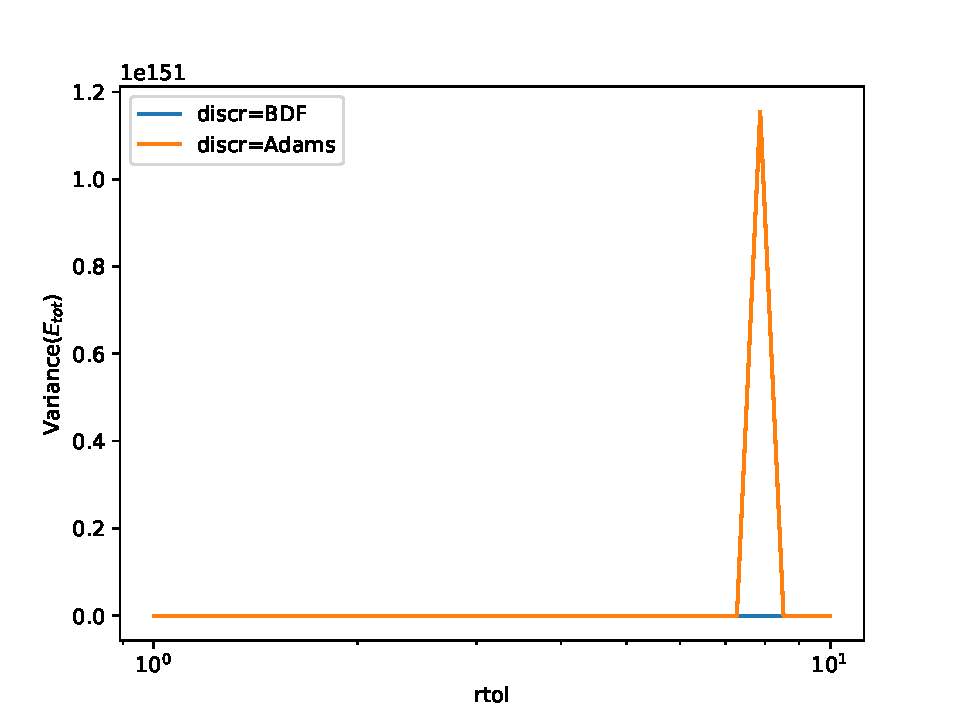
\includegraphics[width=\textwidth]{../Plots/Task4/Figure_304}
\caption{Variance of the energy in relation to the parameter \pyth{rtol}.}
\label{pl:stability2}
\end{minipage}
\end{figure}

\newpage

\subsection*{Testing the parameter atol}

\begin{wrapfigure}{r}{0.45\textwidth}
\centering
\vspace*{-0.8cm}
\begin{minipage}[t]{0.45\textwidth}
\centering
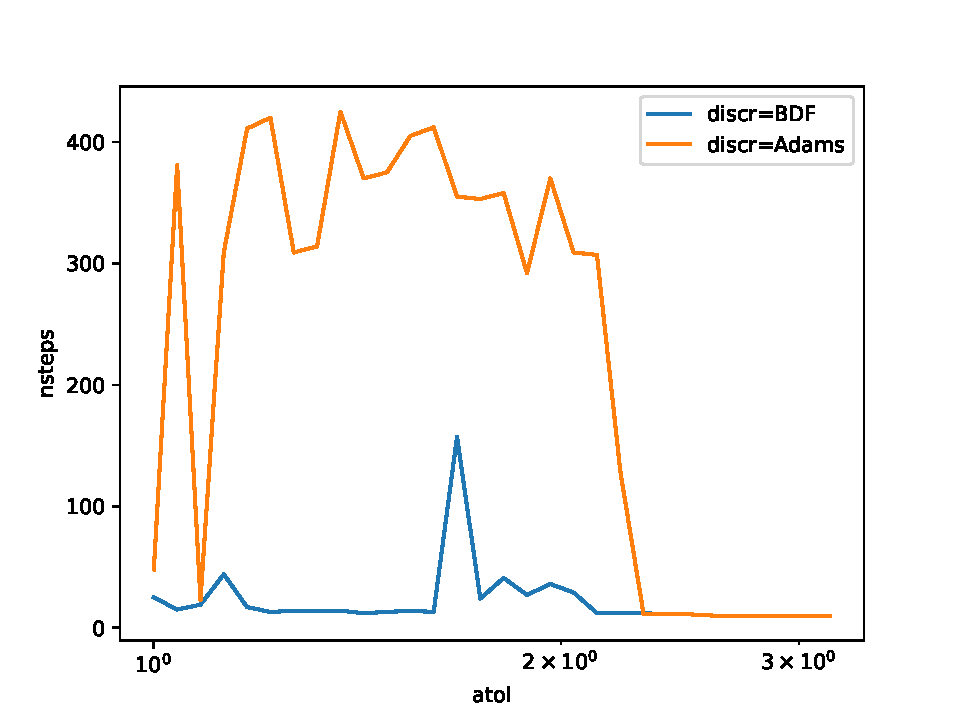
\includegraphics[width=\textwidth]{../Plots/Task4/Figure_400}
\caption{\pyth{nsteps} in relation to the parameter \pyth{atol}.}
\label{pl:nsteps3}
\end{minipage}
\vspace*{0.5cm}
\end{wrapfigure}

\begin{figure}[h]
\centering
\begin{minipage}[t]{0.45\textwidth}
\centering
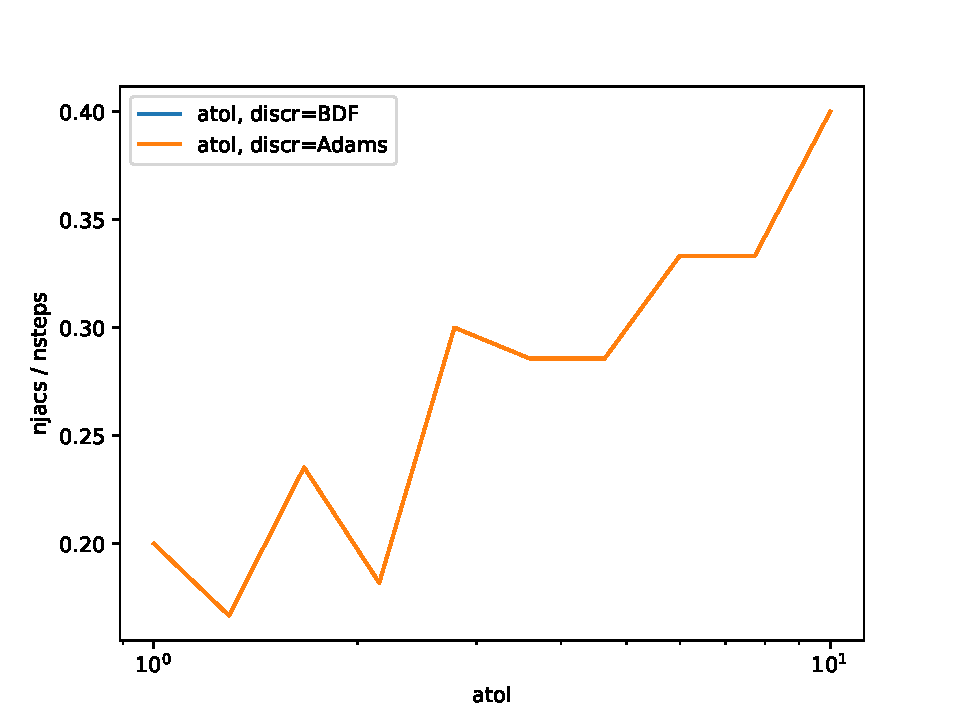
\includegraphics[width=\textwidth]{../Plots/Task4/Figure_411}
\caption{\pyth{njacs/nsteps} in relation to the parameter \pyth{atol}.}
\label{pl:njacs_nsteps3}
\end{minipage}
\hfill
\begin{minipage}[t]{0.45\textwidth}
\centering
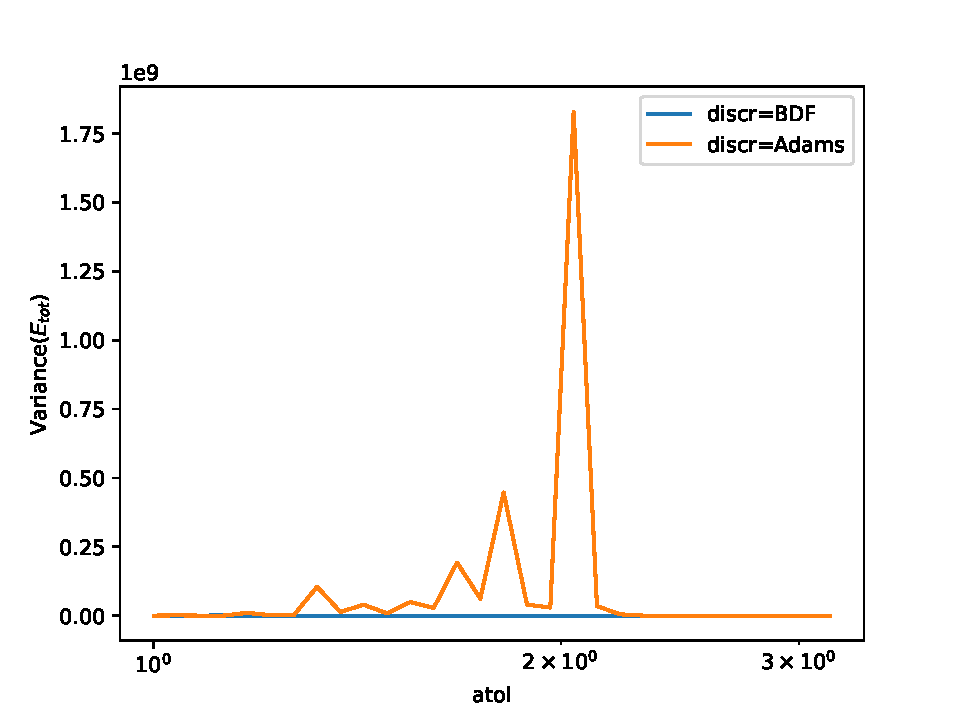
\includegraphics[width=\textwidth]{../Plots/Task4/Figure_404}
\caption{Variance of the energy in relation to the parameter \pyth{atol}.}
\label{pl:stability3}
\end{minipage}
\end{figure}


When testing the \pyth{atol} analogously to the parameter \pyth{rtol} one observes similar behaviour. As \pyth{atol} increases the number of steps taken dramatically decreases (figure \ref{pl:nsteps3}), the number of jacobian evaluations per step eventually increases (figure \ref{pl:njacs_nsteps3} and for the Adams-Moulton method the variance of the total energy also eventually increases (figure \ref{pl:stability3}). Here again a larger value for the variance of the total energy indicates instability.
In either case we observe that increasing the tolerance seems to come at the cost of energy conversation as is dramatically visualised in figures \ref{pl:energy2} and \ref{pl:energy3}.



\begin{figure}[h]
\centering
\begin{minipage}[t]{0.45\textwidth}
\centering
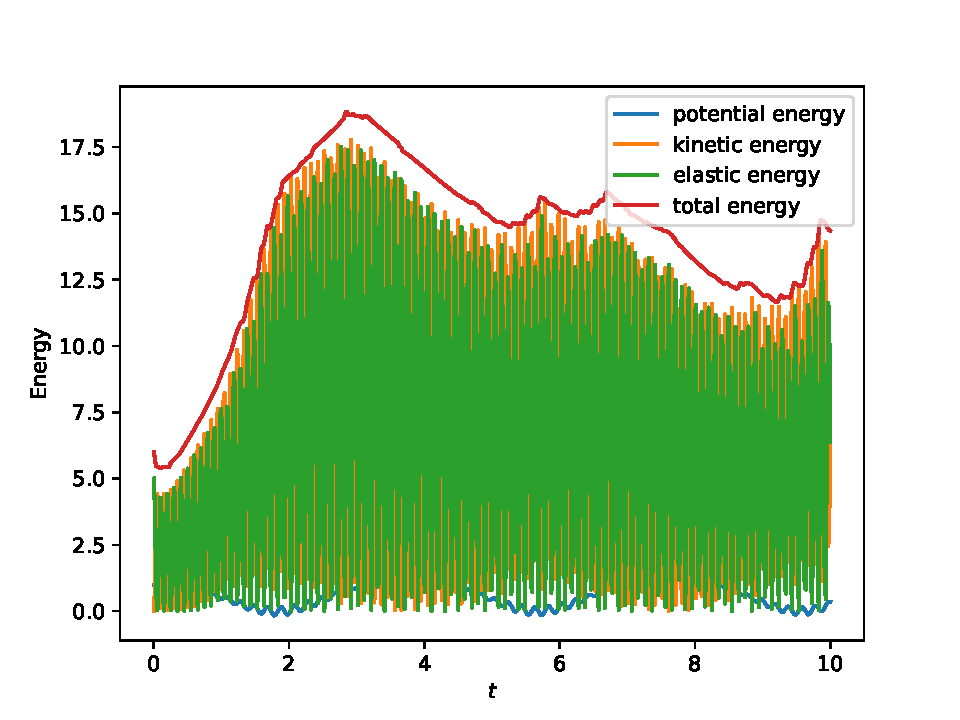
\includegraphics[width=\textwidth]{../Plots/Task4/Figure_450}
\caption{Energy plot for $k=10^3$ with \pyth{atol=1E-2}.}
\label{pl:energy2}
\end{minipage}
\hfill
\begin{minipage}[t]{0.45\textwidth}
\centering
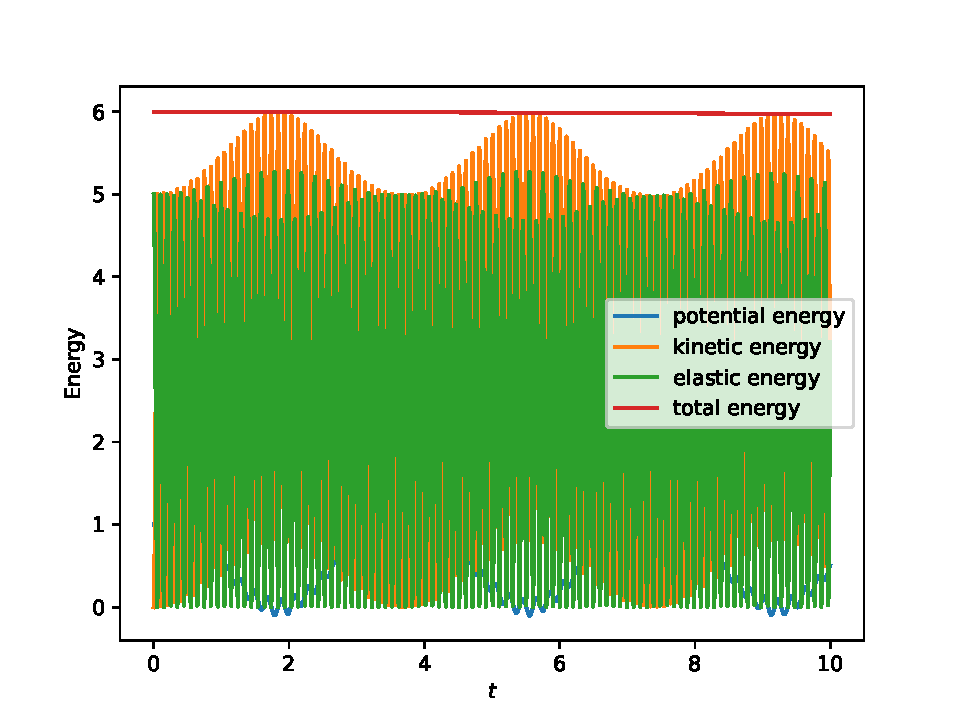
\includegraphics[width=\textwidth]{../Plots/Task4/Figure_451}
\caption{Energy plot for $k=10^3$.}
\label{pl:energy3}
\end{minipage}
\end{figure}

\newpage
All in all we see that none of the (admittedly crude) tweaking of the parameters improved the performance of CVODE. To the contrary, most changes worsened the performance. The choice of the discretisation method on the other hand did make a big difference and the performance for solving the toy problem could be improved by switching from the default BDF method to the Adams-Moulton method.


\chapter*{Project 2}

In this project we used the implementation of the seven body mechanism as described in \cite{HW_SolvingODEs} to test Assimulo's implicit solvers. The problem formulation leads to an index 3 problem of the form
\begin{align}
	M(q)\,q''&= f(q,q')-G(q)^\top\,\lambda\label{eq:sevenBody} \\
	0 &= g(q) \label{eq:condition_indx3}
\end{align}
where $q\in\R^7$, $\lambda\in\R^6$ and $G=Dg$. If we differentiate condition \eqref{eq:condition_indx3} we obtain the index 2 condition
\begin{align*}
	0&=G(q)\,q'
\end{align*}
and differentiating this again we obtain the index 1 formulation
\begin{align}
	0&= \partial_q^2g(q)\,(q',q')+G(q)\,q''\,.  \label{eq:condition_indx1}
\end{align}
\begin{figure}[b]
\centering
\begin{minipage}[t]{0.45\textwidth}
\centering
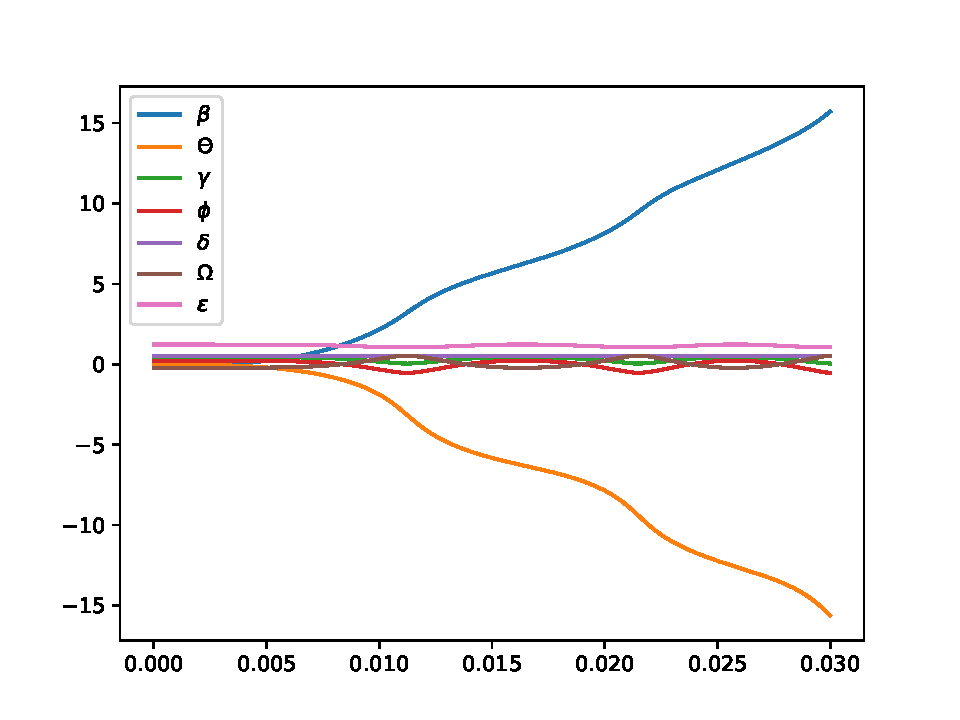
\includegraphics[width=\textwidth]{../Plots/Project2_main/Figure_510}
\caption{The angles of the solution to the index 2 problem.}
\label{pl:indx3_soln_angles}
\end{minipage}
\hfill
\begin{minipage}[t]{0.45\textwidth}
\centering
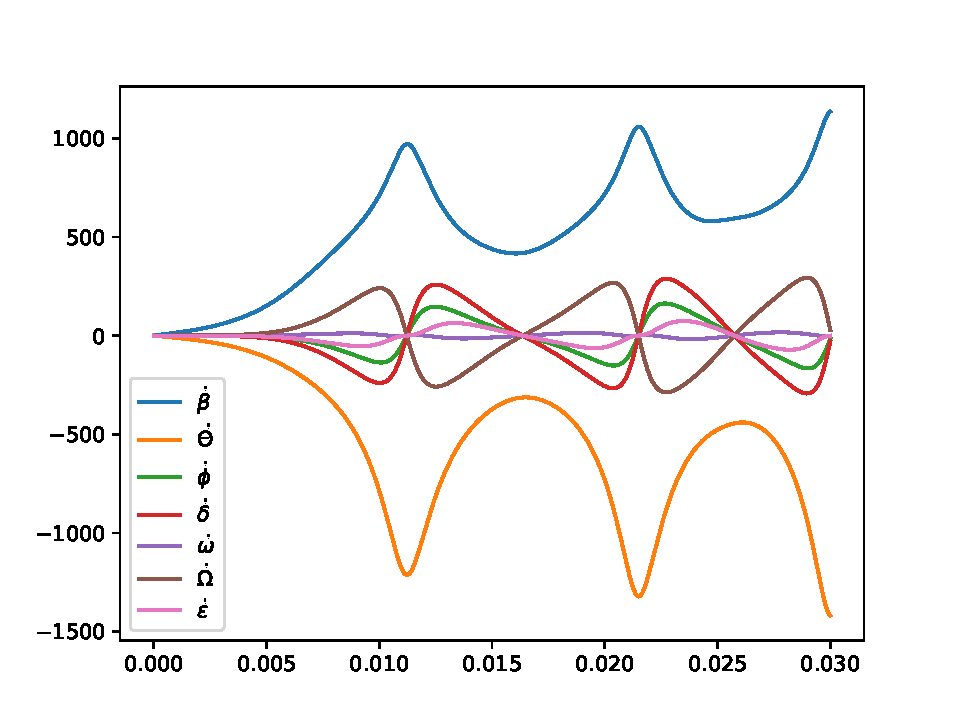
\includegraphics[width=\textwidth]{../Plots/Project2_main/Figure_511}
\caption{The angle speed of the solution to the index 2 problem.}
\label{pl:indx3_soln_anglesdot}
\end{minipage}
\end{figure}
Note that condition \eqref{eq:condition_indx1} and \eqref{eq:sevenBody} can be uniquely solved for $q''$ and $\lambda$ and we then obtain an ODE in the explicit formulation.
For the implementation we rewrite this second order system as a first order system by the usual trick of introducing the variable $v=q'$ so that in the implicit formulation the problem depends on the variable
\begin{align*}
	y = \vect{q \\ v \\ \lambda}\,.
\end{align*}
A plot of the solution of the index 1 formulation can be seen in figures \ref{pl:indx3_soln_angles} to \ref{pl:indx3_soln_lambdas}.

\begin{figure}[t]
\centering
\begin{minipage}[b]{0.45\textwidth}
\centering
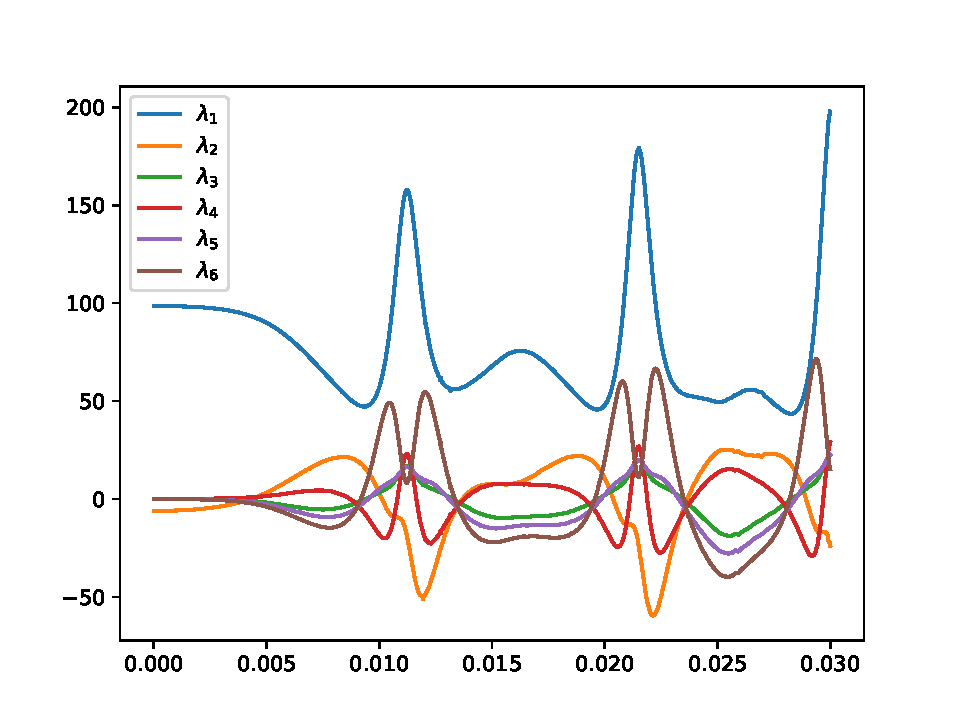
\includegraphics[width=\textwidth]{../Plots/Project2_main/Figure_512}
\caption{The Lagrange parameter of the solution to the index 2 problem.}
\label{pl:indx3_soln_lambdas}
\end{minipage}
\end{figure}



\section*{Generation of consistent initial values}

Due to the restrictions imposed on the system the generation of initial values is no trivial task. To do this we follow the steps presented in \cite{HW_SolvingODEs}. We start with $q$ and $v$.


\begin{figure}[h]
\centering
\begin{minipage}[b]{0.3\textwidth}
\centering
\begin{tabular}{lr}
\hline
 \$\textbackslash{}beta\$    & -0.0617139 \\
 \$\textbackslash{}Theta\$   &  0         \\
 \$\textbackslash{}gamma\$   &  0.45528   \\
 \$\textbackslash{}phi\$     &  0.222668  \\
 \$\textbackslash{}delta\$   &  0.487365  \\
 \$\textbackslash{}Omega\$   & -0.222668  \\
 \$\textbackslash{}epsilon\$ &  1.23055   \\
\hline
\end{tabular}
\caption{Consistent initial angles}
\label{tb:initial_angles}
\end{minipage}
\hfill
\begin{minipage}[b]{0.3\textwidth}
\centering
\begin{tabular}{lr}
\hline
 \$\textbackslash{}ddot\{\textbackslash{}beta\}\$    &  14222.4         \\
 \$\textbackslash{}ddot\{\textbackslash{}Theta\}\$   & -10666.8         \\
 \$\textbackslash{}ddot\{\textbackslash{}phi\}\$     &      7.58763e-14 \\
 \$\textbackslash{}ddot\{\textbackslash{}delta\}\$   &      3.22329e-13 \\
 \$\textbackslash{}ddot\{\textbackslash{}omega\}\$   &      7.02222e-13 \\
 \$\textbackslash{}ddot\{\textbackslash{}Omega\}\$   &     -3.22329e-13 \\
 \$\textbackslash{}ddot\{\textbackslash{}epsilon\}\$ &      8.6019e-13  \\
\hline
\end{tabular}
\caption{Consistent initial accelerations}
\label{tb:initial_accelerations}
\end{minipage}
\hfill
\begin{minipage}[b]{0.3\textwidth}
\centering
\begin{tabular}{lr}
\hline
 $\lambda_1$ & 98.5669      \\
 $\lambda_2$ & -6.12269     \\
 $\lambda_3$ &  2.2899e-17  \\
 $\lambda_4$ & -1.87294e-17 \\
 $\lambda_5$ &  3.37745e-17 \\
 $\lambda_6$ &  4.83113e-17 \\
\hline
\end{tabular}
\caption{Consistent initial lambdas}
\label{tb:initial_lambdas}
\end{minipage}
\end{figure}

First we take $\theta=0$ which can be done given that the system is under-determined under the assumption that a solution exists (this makes sense as a physical model of the system was presented in class). We then use \textit{Newton Iteration} to solve the equations obtaining values for the remaining angles.
We also take the initial value of $v$ to be $0$ as we assume the system starts at rest. Now for $w$ and $\lambda$ using the Index 1 formulation we have to solve a linear system which is presented in \cite{HW_SolvingODEs}. Doing this we get the values given in tables  \ref{tb:initial_angles}, \ref{tb:initial_accelerations} and \ref{tb:initial_lambdas}.
Many of the values are minute but non-zero. This is due to rounding errors, but in theory these small values equal zero.

\section*{A comparison of the index 1, 2 and 3 formulations}

\begin{figure}[h]
\centering
\begin{minipage}[t]{0.45\textwidth}
\centering
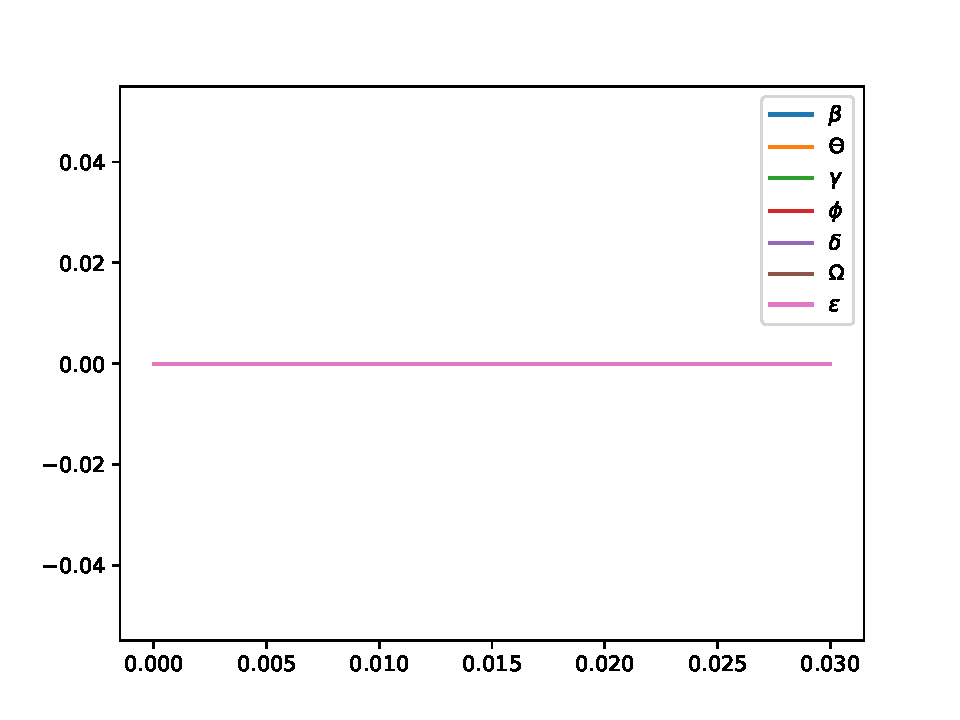
\includegraphics[width=\textwidth]{../Plots/Project2_main/Figure_530}
\caption{The difference of angles of the index 1 and the index 3 solution.}
\label{pl:indx1_solndiff_angles}
\end{minipage}
\hfill
\begin{minipage}[t]{0.45\textwidth}
\centering
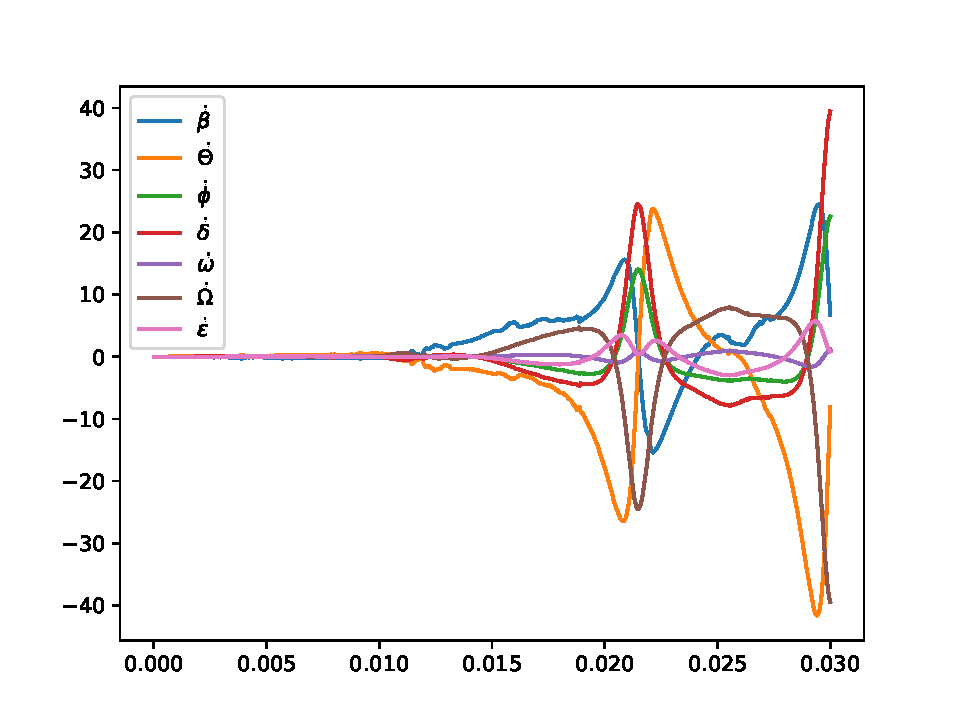
\includegraphics[width=\textwidth]{../Plots/Project2_main/Figure_531}
\caption{The difference in angle speeds of the index 1 and the index 3 solution.}
\label{pl:indx1_solndiff_anglesdot}
\end{minipage}
\end{figure}

\begin{figure}[h]
\centering
\begin{minipage}[t]{0.45\textwidth}
\centering
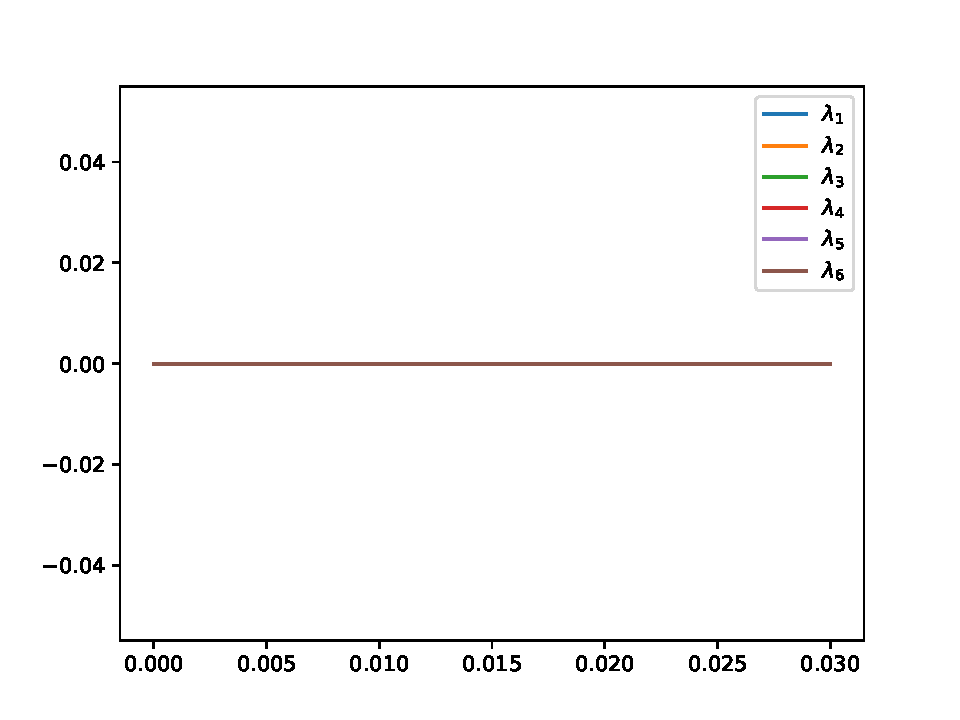
\includegraphics[width=\textwidth]{../Plots/Project2_main/Figure_532}
\caption{The difference of lambdas of the index 1 and the index 3 solution.}
\label{pl:indx1_solndiff_lambdas}
\end{minipage}
\hfill
\begin{minipage}[t]{0.45\textwidth}
\centering
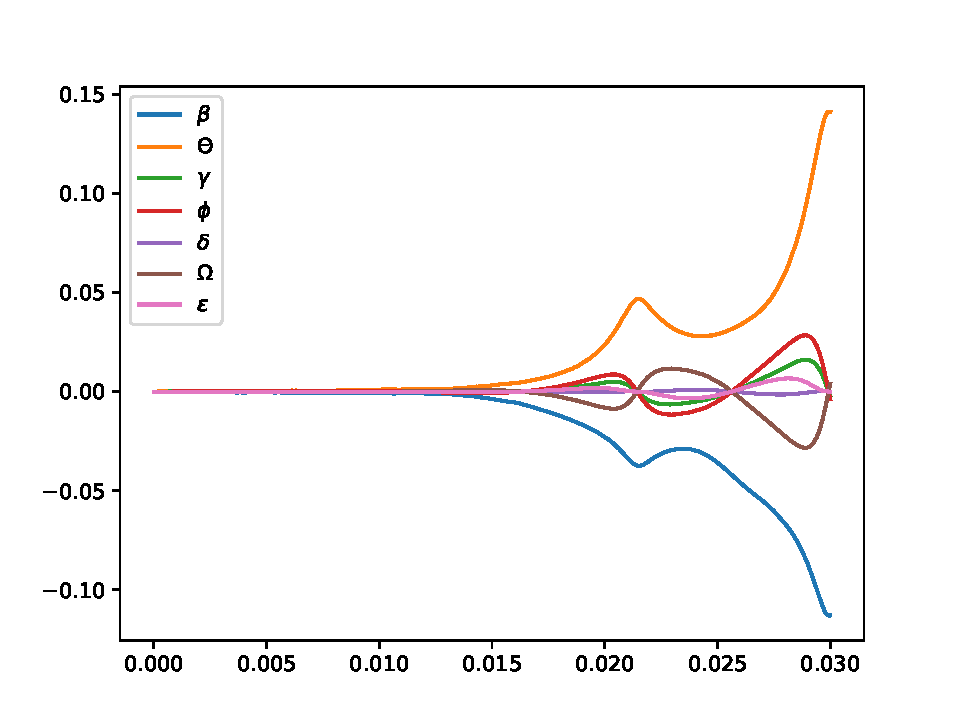
\includegraphics[width=\textwidth]{../Plots/Project2_main/Figure_540}
\caption{The difference of angles of the index 2 and the index 3 solution.}
\label{pl:indx2_solndiff_angles}
\end{minipage}
\end{figure}

We now will compare the solutions of the different formulations. To calculate the solutions we used the IDA solver. To get the problem to run we set the \pyth{atol} parameter to the large number \pyth{1E5} and the \pyth{algvar} parameter to \pyth{False} for the algebraic variable $\lambda$ and for $v$. These settings remain unchanged and in the following we only vary the index of the problem. One can see in the figures \ref{pl:indx1_solndiff_angles} to \ref{pl:indx1_solndiff_lambdas}  the index 1 solution subtracted from the index 3 solution. In figures \ref{pl:indx2_solndiff_angles} to \ref{pl:indx2_solndiff_lambdas} we see the index 2 solution subtracted from the index 3 solution. As expected we see that the difference the solutions grows as time progresses.


\begin{figure}[h]
\centering
\begin{minipage}[t]{0.45\textwidth}
\centering
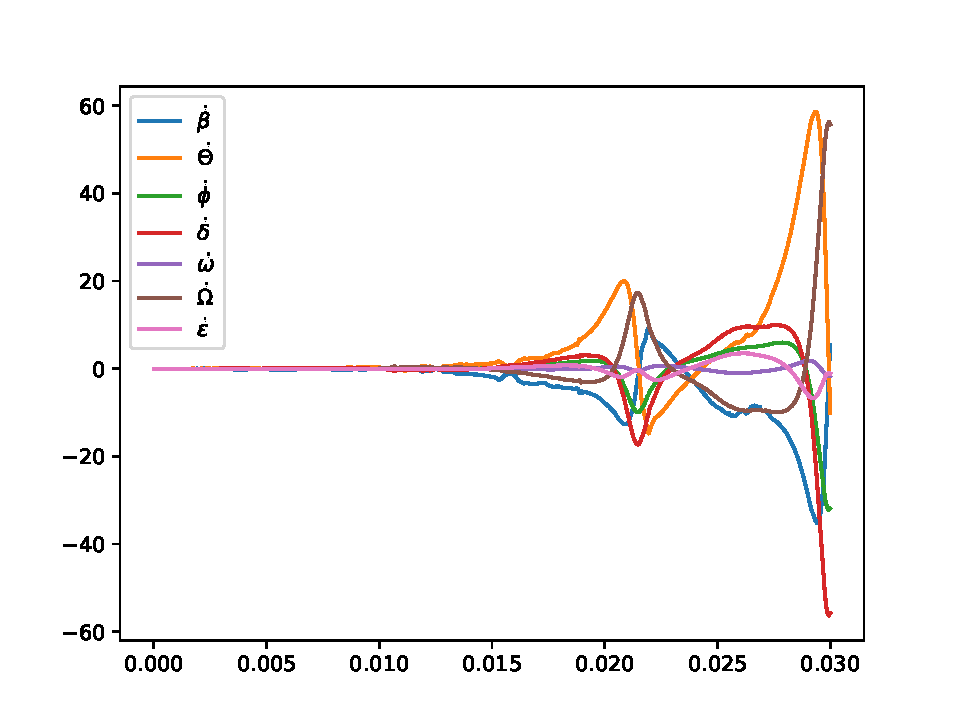
\includegraphics[width=\textwidth]{../Plots/Project2_main/Figure_541}
\caption{The difference in angle speeds of the index 2 and the index 3 solution.}
\label{pl:indx2_solndiff_anglesdot}
\end{minipage}
\hfill
\begin{minipage}[t]{0.45\textwidth}
\centering
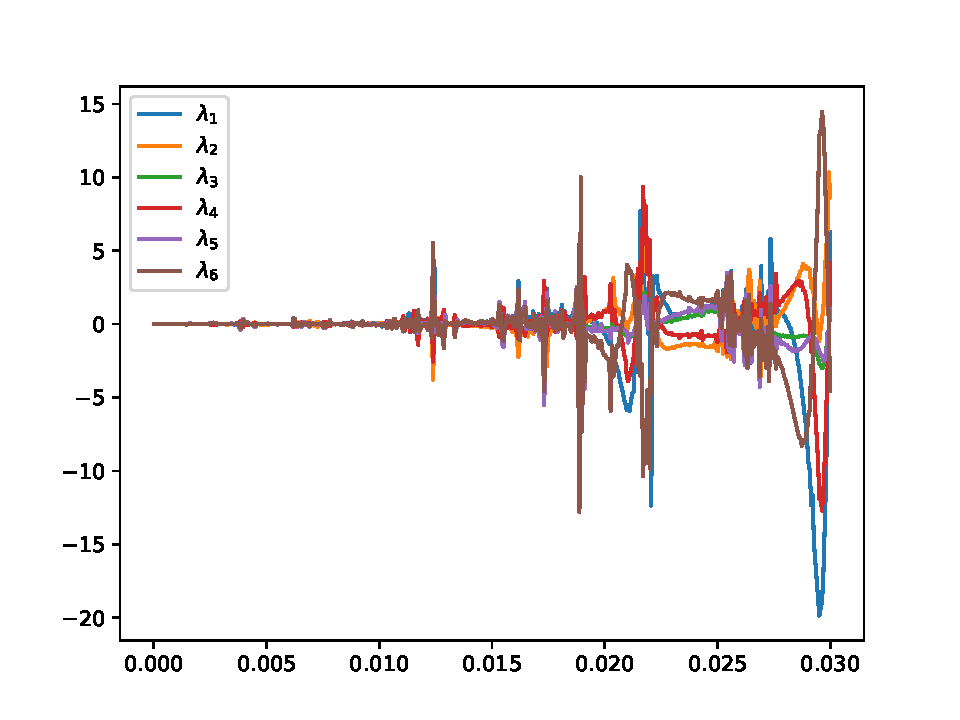
\includegraphics[width=\textwidth]{../Plots/Project2_main/Figure_542}
\caption{The difference of lambdas of the index 2 and the index 3 solution.}
\label{pl:indx2_solndiff_lambdas}
\end{minipage}
\end{figure}

\begin{figure}[h]
\centering
\begin{minipage}[t]{0.45\textwidth}
\centering
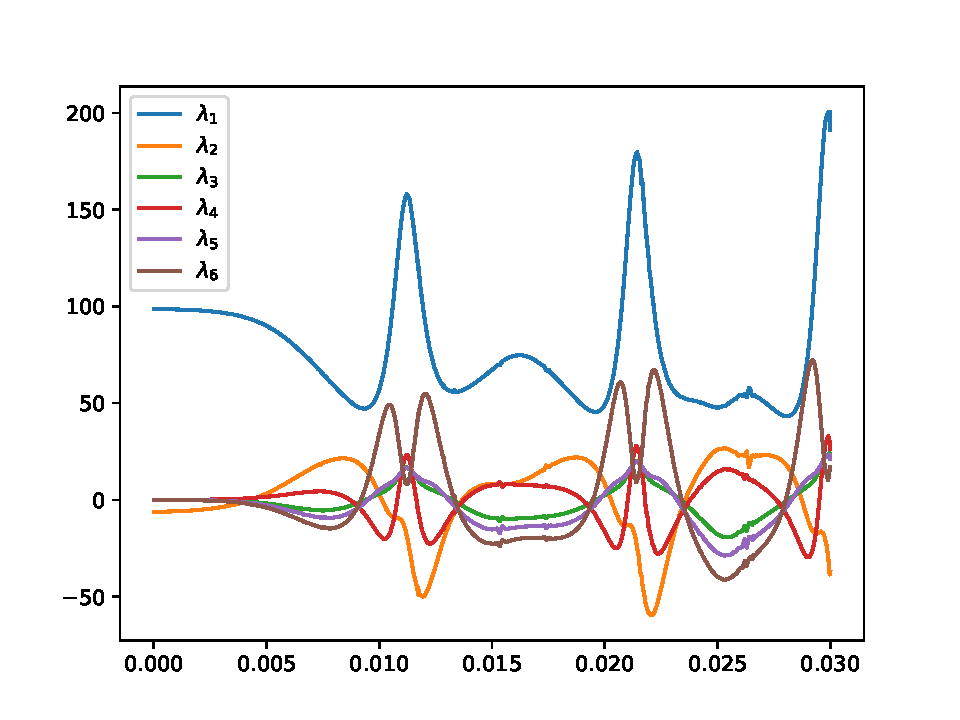
\includegraphics[width=\textwidth]{../Plots/Project2_main/Figure_515}
\caption{The Lagrange parameter of the index 2 problem.}
\label{pl:indx1_soln_lambdas}
\end{minipage}
\hfill
\begin{minipage}[t]{0.45\textwidth}
\centering
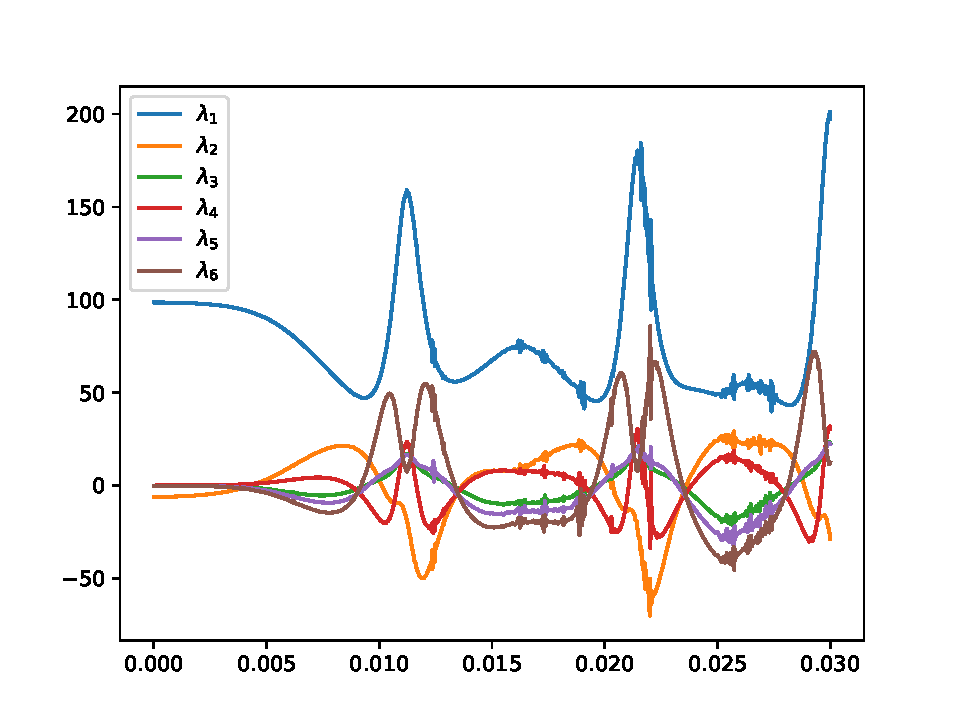
\includegraphics[width=\textwidth]{../Plots/Project2_main/Figure_518}
\caption{The Lagrange parameter of the index 3 problem.}
\label{pl:indx2_soln_lambdas}
\end{minipage}
\end{figure}

Rather unexpectedly the difference of the index 1 to the index 3 solution is in general greater than the difference of the index 2 to the index 3 solutions. Also unexpectedly these differences are noticeable in the plots of the Lagrange parameter $\lambda$ as shown in figures \ref{pl:indx1_soln_lambdas}, \ref{pl:indx2_soln_lambdas} and \ref{pl:indx3_soln_lambdas}. Here we see that the solution becomes increasingly rough as the index increases.



The performance of the IDA solver for the various indexes can be seen in figures \ref{pl:nsteps_indx123} to \ref{pl:nerrfails_nsteps_indx123}. We see in figure \ref{pl:nsteps_indx123} that the number of steps of the solver increases with the index. As the number of function evaluations per step stays roughly constant (c.f.\ figure \ref{pl:nfcns_nsteps_indx123}) this means that the number of function evaluations increases with the index.
In the number of error test failures (figure \ref{pl:nerrfails_nsteps_indx123}) we see a larger difference between the problems though this is probably not statistically significant as the total number of error test failures is approximately a dozen.
\newpage

\begin{figure}[h]
\centering
\begin{minipage}[t]{0.3\textwidth}
\centering
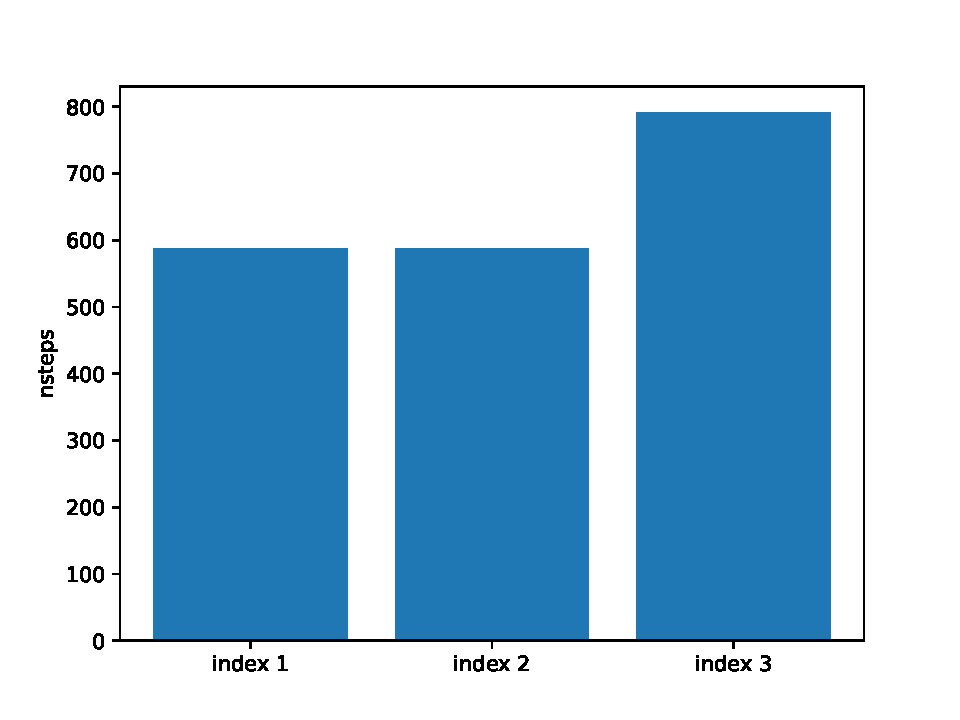
\includegraphics[width=\textwidth]{../Plots/Project2_main/Figure_600}
\caption{\pyth{nsteps} in relation to the index.}
\label{pl:nsteps_indx123}
\end{minipage}
\hfill
\begin{minipage}[t]{0.3\textwidth}
\centering
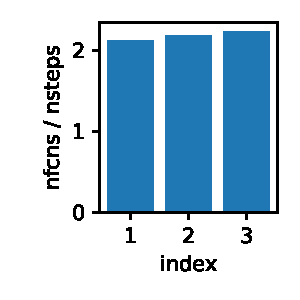
\includegraphics[width=\textwidth]{../Plots/Project2_main/Figure_610}
\caption{\pyth{nfcns/nsteps} in relation to the index.}
\label{pl:nfcns_nsteps_indx123}
\end{minipage}
\hfill
\begin{minipage}[t]{0.3\textwidth}
\centering
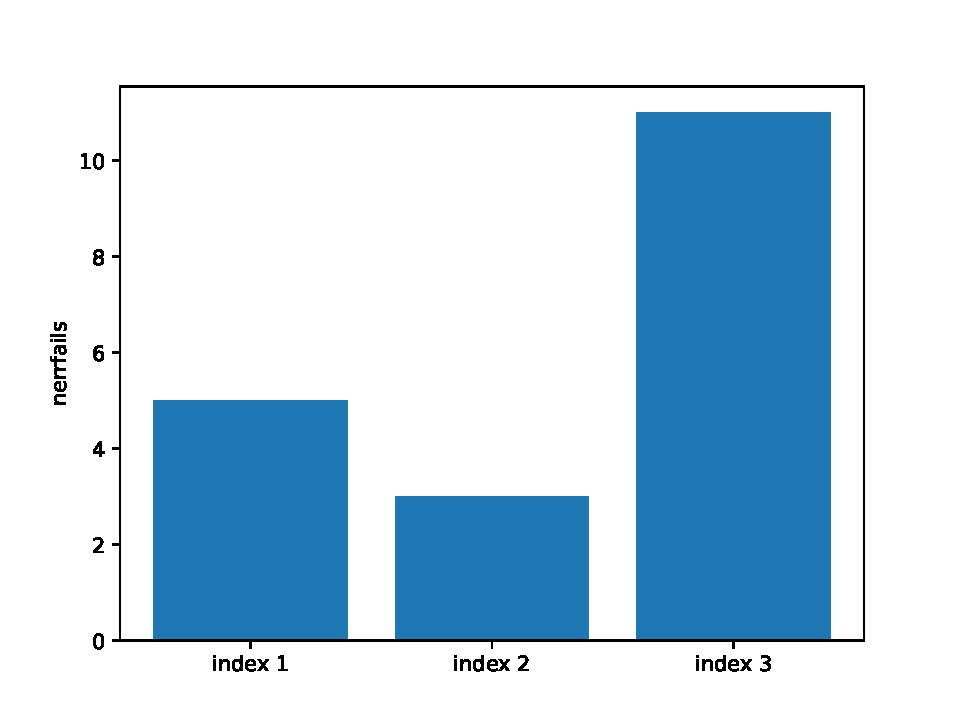
\includegraphics[width=\textwidth]{../Plots/Project2_main/Figure_603}
\caption{\pyth{nerrfails} in relation to the index.}
\label{pl:nerrfails_indx123}
\end{minipage}
\end{figure}


\begin{figure}[h]
\centering
\begin{minipage}[b]{0.3\textwidth}
\centering
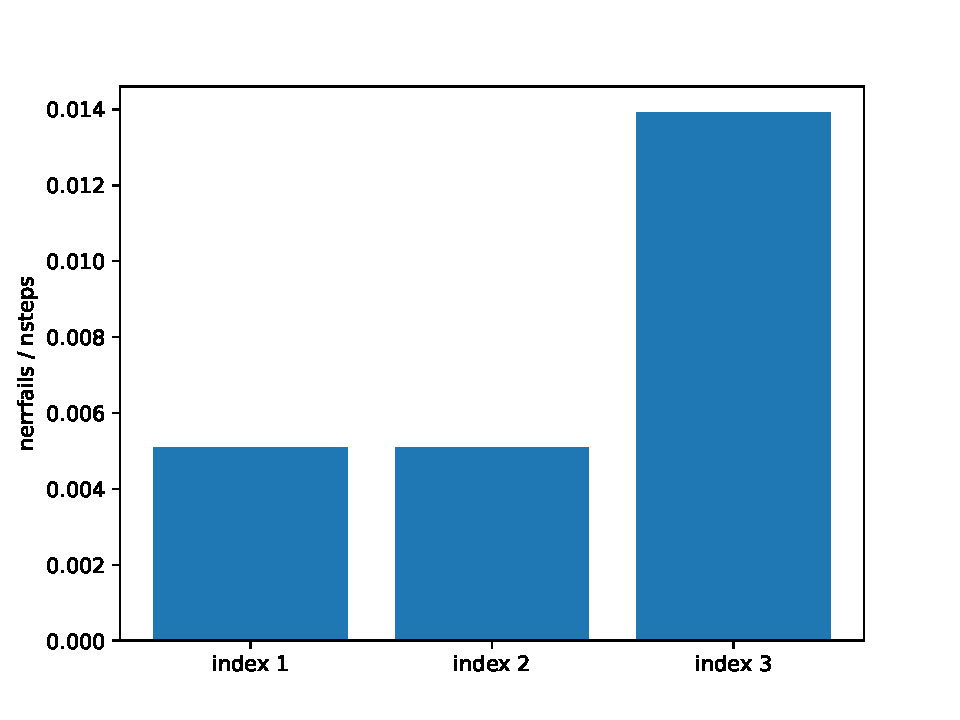
\includegraphics[width=\textwidth]{../Plots/Project2_main/Figure_612}
\caption{\pyth{nerrfails/nsteps} in relation to the index.}
\label{pl:nerrfails_nsteps_indx123}
\end{minipage}
\end{figure}

\vspace*{-0.5cm}

\section*{Dependence on the parameters \pyth{algvar} and \pyth{atol}}

As previously indicated the IDA solver will throw an error
\begin{python}
assimulo.solvers.sundials.IDAError: 'Convergence test failures occurred too many times during one internal time step or minimum step size was reached. At time 0.000000.'
\end{python}
This can be resolved by declaring the entries of $y$ corresponding to $v$ and or $\lambda$ to be algebraic variables with the parameter \pyth{algvar} and to set the parameter \pyth{atol} to a large constant. In the following we will check how these parameters impact the performance of the solver for the index 1 formulation. For this denote by \pyth{algvar_v} and \pyth{algvar_lambda} the value of the \pyth{algvar} parameter for $v$ and $\lambda$. The default value of \pyth{algvar} is set to \pyth{True}. Analogously denote the components of \pyth{atol} corresponding to $v$ and $\lambda$ with \pyth{atol_v} and \pyth{atol_lambda} and set the default value to \pyth{1E-6}. We run a series of 5 experiments as depicted in table \ref{tb:indx1_experiment_params}.


\begin{figure}[h]
\centering
{\footnotesize
\begin{tabular}{rrrrlll}
\hline
   experiment &   index &     atol\_v &   atol\_lambda & algvar\_v   & algvar\_lambda   & suppress\_alg   \\
\hline
            0 &       1 & 100000     &    100000     & False      & False           & True           \\
            1 &       1 &      1e-06 &    100000     & False      & True            & True           \\
            2 &       1 &      1e-06 &    100000     & True       & False           & True           \\
            3 &       1 &      1e-06 &    100000     & True       & True            & False          \\
            4 &       1 &      1e-06 &         1e-06 & False      & False           & True           \\
\hline
\end{tabular}
}
\caption{Parameters in the experiments}
\label{tb:indx1_experiment_params}
\end{figure}

As all experiments deliver a similar result we will compare the statistics of IDA as depicted in figures \ref{pl:nsteps_indx1} to \ref{pl:nerrfails_nsteps_indx1}. Once again we observe in figure \ref{pl:nfcns_nsteps_indx1} that the total number of function evaluations is roughly proportional to the number of steps. Here experiments 1 and 4 stick out for requiring comparatively more function evaluations per step. However in figure \ref{pl:nsteps_indx1} we see that these are also precisely the experiments in which the total number of steps taken is by far the least. Experiments 1 and 4 are also precisely those experiments that have the most stringent requirements on the $v$ part of $y$. Both have set \pyth{atol_v=1E-6} and declare $v$ to not be an algebraic variable. We see in figures \ref{pl:njacs_indx1} and \ref{pl:nerrfails_nsteps_indx1} that experiment 0 is an outlier in requiring comparatively many Jacobian evaluations and having relatively few error test failures.

\begin{figure}[h]
\centering
\begin{minipage}[t]{0.3\textwidth}
\centering
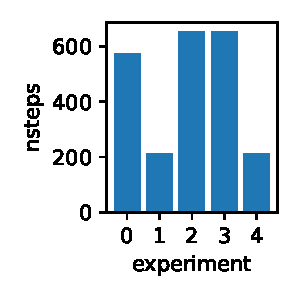
\includegraphics[width=\textwidth]{../Plots/Project2_main/Figure_700}
\caption{\pyth{nsteps} of the experiments.}
\label{pl:nsteps_indx1}
\end{minipage}
\hfill
\begin{minipage}[t]{0.3\textwidth}
\centering
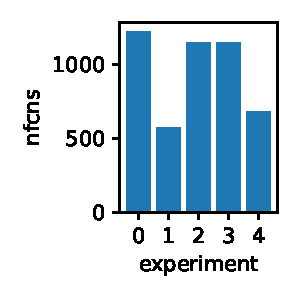
\includegraphics[width=\textwidth]{../Plots/Project2_main/Figure_701}
\caption{\pyth{nfcns}  of the experiments.}
\label{pl:nfcns_indx1}
\end{minipage}
\hfill
\begin{minipage}[t]{0.3\textwidth}
\centering
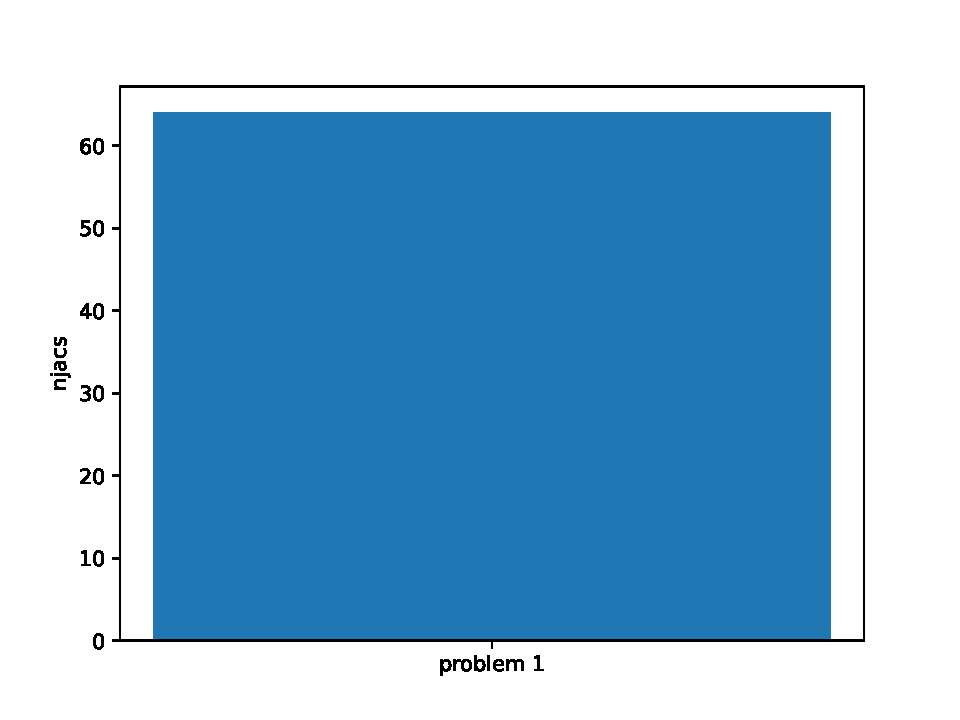
\includegraphics[width=\textwidth]{../Plots/Project2_main/Figure_702}
\caption{\pyth{njacs}  of the experiments.}
\label{pl:njacs_indx1}
\end{minipage}
\end{figure}


\begin{figure}[b]
\centering
\begin{minipage}[t]{0.3\textwidth}
\centering
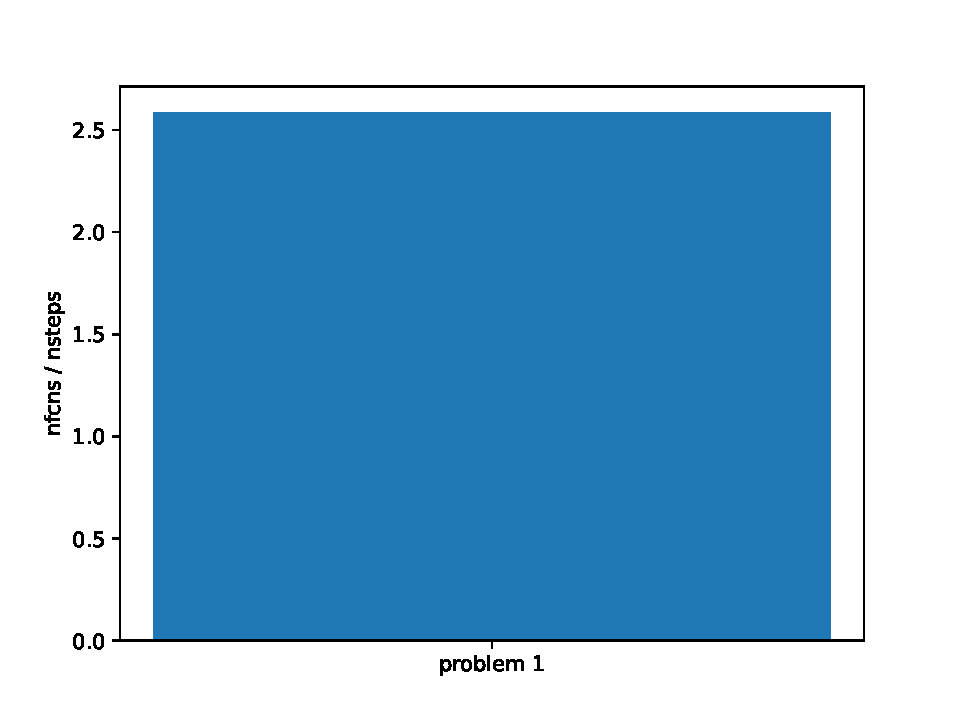
\includegraphics[width=\textwidth]{../Plots/Project2_main/Figure_710}
\caption{\pyth{nfcns/nsteps} of the experiments.}
\label{pl:nfcns_nsteps_indx1}
\end{minipage}
\hfill
\begin{minipage}[t]{0.3\textwidth}
\centering
\includegraphics[width=\textwidth]{../Plots/Project2_main/Figure_711}
\caption{\pyth{njacs/nsteps} of the experiments.}
\label{pl:njacs_nsteps_indx1}
\end{minipage}
\hfill
\begin{minipage}[t]{0.3\textwidth}
\centering
\includegraphics[width=\textwidth]{../Plots/Project2_main/Figure_712}
\caption{\pyth{nerrfails/nsteps} of the experiments.}
\label{pl:nerrfails_nsteps_indx1}
\end{minipage}
\end{figure}

\section*{Using an explicit method}

As part of the final task we used an explicit RK4 method to solve the index 1 problem. As a result of the method exploding for $h=0.01$, the default step value, the method was tested for various values of $h$.

In figure  \ref{pl:L2_norm_explicit} the $L_2$ norm of each angle over time is plotted with respect to $h \in [0.001, 0.002)$ with $\Delta h = 5\mathrm{e}{-6}$.

\begin{figure}[h]
\centering
\begin{minipage}[t]{0.7\textwidth}
\centering
\includegraphics[width=\textwidth]{../Plots/RK4_Proj2/L2_norm_different_k.pdf}
\caption{Value of $L_2$ norms depending on $h$}
\label{pl:L2_norm_explicit}
\end{minipage}
\end{figure}


The explicit method can then be tested with individual step sizes and as expected, the method explodes e.g.\ for $h \in \{0.001446, 0.0018, 0.00195\}$ and is stable for $h \in \{0.00185, 0.0012, 0.0016\}$.

In figures \ref{pl:explicit_angles}  and \ref{pl:explicit_angles_dot} the approximation using the explicit RK4 with the stable step size $h=10^{-4}$ can be observed.

\begin{figure}[h]
\centering
\begin{minipage}[t]{0.45\textwidth}
\centering
\includegraphics[width=\textwidth]{../Plots/RK4_Proj2/angles}
\caption{Approximation of angles using explicit method}
\label{pl:explicit_angles}
\end{minipage}
\hfill
\begin{minipage}[t]{0.45\textwidth}
\centering
\includegraphics[width=\textwidth]{../Plots/RK4_Proj2/derivatives}
\caption{Approximation of angles derivatives using explicit method}
\label{pl:explicit_angles_dot}
\end{minipage}
\end{figure}

\chapter*{Project 3}

In this project we consider an initial value problem of the form
\begin{align}
	\begin{aligned}
	M \ddot{u}+C\dot{u}+Ku &= f(t) \\
	u(0) &= u_0 \\
	\dot{u}(0) &= v_0
	\end{aligned}
	\label{eq:IVPSparse}
\end{align}
where $M, C, K\in\R^{n\times n}$ are sparse matrices and $u_0, v_0\in\R^n$ initial values. For this we implemented an Assimulo problem class, the HHT solver and the Newmark implicit and explicit solvers. The explicit solver was tested on the pendulum. The implicit solvers were tested on a discretised PDE obtained from an elastic beam which yields a system of the form \eqref{eq:IVPSparse}.

We will see that Newmark's method handles sparse systems much more efficiently than some Assimulo solvers.
We will also see the dependence of the stability of Newmark's implicit method on the parameters $\beta$ and $\gamma$ and the dependence of the HHT method on the parameter $\alpha$ which should be chosen carefully for a given problem.

\section*{The elastic pendulum revisited}

In this section we will use the aforementioned methods to solve the problem of the elastic spring from Project 1. In particular we will compare the performance of different explicit methods for solving the problem. We will compare Newmark Explicit with Explicit Euler and Newmark Explicit with RK4.

It is common to both methods that the simulations starts at the same point and rapidly drifts away. This drift will continue in different ways depending on the method tested.

\subsection*{Newmark - RK4}

This is probably the most interesting of both cases given that RK4 does not lose stability as quickly as Explicit Euler does. The distance between the approximations will dilate in an oscillating manner with increasing amplitude. This can be observed in figure \ref{pl:new_rk4_k=10} for $y$ and in figure \ref{pl:new_rk4_k=10_dot} for $\dot{y}$.

\begin{figure}[h]
\centering
\begin{minipage}[t]{0.45\textwidth}
\centering
\includegraphics[width=\textwidth]{../Plots/Diff_Proj3/Real/New-RK4_k=1E1_t=1E5_y}
\caption{Difference of $y$ with $h=0.01$ and $k=10$.}
\label{pl:new_rk4_k=10}
\end{minipage}
\hfill	
\begin{minipage}[t]{0.45\textwidth}
\centering
\includegraphics[width=\textwidth]{../Plots/Diff_Proj3/Real/New-RK4_k=1E1_t=1E5_ydot}
\caption{Difference of $\dot{y}$ with $h=0.01$ and $k=10$.}\label{pl:new_rk4_k=10_dot}
\end{minipage}
\end{figure}

The amplitude of the oscillations will eventually converge to a value which appears to depend on the value of $k$. For bigger values of $k$ the amplitude appears to converge faster. Convergence of the amplitudes can be observed in figure \ref{pl:new_rk4_k=1000} for $y$ and in figure \ref{pl:new_rk4_k=1000_dot} for $\dot{y}$.

\begin{figure}[h]
\centering
\begin{minipage}[t]{0.45\textwidth}
\centering
\includegraphics[width=\textwidth]{../Plots/Diff_Proj3/Real/New-RK4_k=1E3_t=1E5_y}
\caption{Difference of $y$ with $h=0.01$ and $k=1\mathrm{e}{3}$.}
\label{pl:new_rk4_k=1000}
\end{minipage}
\hfill
\begin{minipage}[t]{0.45\textwidth}
\centering
\includegraphics[width=\textwidth]{../Plots/Diff_Proj3/Real/New-RK4_k=1E3_t=1E5_ydot}
\caption{Difference of $\dot{y}$ with $h=0.01$ and $k=1\mathrm{e}{3}$.}
\label{pl:new_rk4_k=1000_dot}
\end{minipage}
\end{figure}

With regards to performance, Newmark's method is around 1 and 5 time faster than RK4.

\subsection*{Newmark - Euler}
Not much can be said about the relation between Newmark's and Euler's methods given the unstable nature of Explicit Euler. Euler's method explodes to infinity while Newmark's remains stable. This can be observed in figure \ref{pl:new_eul}.

\begin{figure}[h]
\vspace*{-1cm}
\centering
\begin{minipage}[t]{0.45\textwidth}
\centering
\includegraphics[width=\textwidth]{../Plots/Diff_Proj3/Real/New-Eul_k=1E1_t=1E3_y}
\caption{Difference of $y$ with $h=0.01$ and $k=10$.}
\label{pl:new_eul}
\end{minipage}
\end{figure}

With regard to performance, Euler's method is around 1 and 5 faster than Newmark's.

\newpage

\section*{An elastic beam}

In the second part of the project we tested the implicit Newmark and the HHT method on a discretised beam plotted in figure \ref{pl:beam_soln_initial}. The beam is displaced by a force until it is deformed as in figure \ref{pl:beam_soln_position1}. With time it then swings back and forth between the positions in figures \ref{pl:beam_soln_initial} to \ref{pl:beam_soln_position3}. Figure \ref{pl:beam_soln_displacement} shows the displacement of the tip of the beam in dependence of time.

\begin{figure}[h]
\begin{minipage}[t]{0.45\textwidth}
\centering
\includegraphics[width=\textwidth]{../Plots/Project3_main/Figure_905.pdf}
\caption{Displacement of the tip of the beam of the solution.}
\label{pl:beam_soln_displacement}
\end{minipage}
\hfill
\centering
\begin{minipage}[t]{0.45\textwidth}
\centering
\includegraphics[width=\textwidth]{../Plots/Project3_main/Figure_902.pdf}
\caption{Energy in dependence of time of the solution.}
\label{pl:beam_soln_energy}
\end{minipage}
\end{figure}

\begin{figure}[h]
\centering
\begin{minipage}[t]{0.45\textwidth}
\centering
\includegraphics[width=\textwidth]{../Plots/Project3_main/Figure_1.pdf}
\caption{Beam position at $t\approx0$.}
\label{pl:beam_soln_initial}
\end{minipage}
\hfill
\begin{minipage}[t]{0.45\textwidth}
\centering
\includegraphics[width=\textwidth]{../Plots/Project3_main/Figure_8.pdf}
\caption{Beam position at $t\approx1.7$.}
\label{pl:beam_soln_position1}
\end{minipage}
\end{figure}

\begin{figure}[h]
\centering
\begin{minipage}[t]{0.45\textwidth}
\centering
\includegraphics[width=\textwidth]{../Plots/Project3_main/Figure_10.pdf}
\caption{Beam position at $t\approx2.4$.}
\label{pl:beam_soln_position2}
\end{minipage}
\hfill
\begin{minipage}[t]{0.45\textwidth}
\centering
\includegraphics[width=\textwidth]{../Plots/Project3_main/Figure_12.pdf}
\caption{Beam position at $t\approx2.7$.}
\label{pl:beam_soln_position3}
\end{minipage}

\end{figure} We can calculate the elastic and kinetic energies according to the formulas
\begin{align*}
	E_{\text{kin}} = \frac{1}{2}v^\top Mv
	\qquad\qquad E_{\text{elast}} = \frac{1}{2}u^\top Cu
\end{align*}
which add up to the total energy
\begin{align*}
	E_{\text{tot}}=E_{\text{kin}}+E_{\text{elast}}\,.
\end{align*}
The development of the energy of the system can be seen in figure \ref{pl:beam_soln_energy}. One can see in particular that after the initial application of an external force to the system the energy remains almost constant. As in project 1 the variance of the total energy serves as a measure of the instability of the solver. Here we calculate this variance only for the latter $4/5$ of the simulation because the applied force changes the total energy in the first part.
With an ideal solver this quantity vanishes.


\subsection*{A brief comparison of solvers}

In a first experiment we compare the performance of our implementation of the HHT solver and the implicit Euler solver from Assimulo. The HHT method was applied with the parameter $\alpha=0$ and the step size $h=0.05$ was identical for both methods. The results are plotted in figure \ref{tb:beam_exp_solverComparison}. One sees that for all solvers the variance of the total energy is small. There is however a big difference in the performance of the methods. On my computer the implicit Euler solver takes roughly two orders of magnitude longer than the HHT method.

\begin{figure}[h]
\centering
\begin{tabular}{lrr}
\hline
 solver                      &   HHT &   ImplicitEuler \\
\hline
 stability\_index             &   0   &             0   \\
 Elapsed simulation time [s] &   1.7 &           224.4 \\
\hline
\end{tabular}
\caption{Performance of various solvers for the beam problem.}
\label{tb:beam_exp_solverComparison}
\end{figure}


\subsection*{Testing the implicit Newmark solver}

In a second experiment we test the dependence of the implicit Newmark method on the parameters $\beta$ and $\gamma$ while keeping the step size $h=0.05$ constant. The variance of the total energy can be seen in figure \ref{pl:beam_exp_betagamma_alpha0}. It should be noted that we cut off the value of the variance of the total energy at $10^2$ because any greater value shows that the solution is unstable for the specific choice of $\beta$ and $\gamma$. One sees that for $1/2\leq \gamma\leq2\beta$ the solver is stable.
Also observe that the solver is most stable for $\gamma\approx1/2$ and for $\beta\approx1/4$ which is precisely the value at which the method achieves second order accuracy. Figure \ref{pl:beam_exp_betagamma_instable1} shows what happens if we leave the region of stability.

\begin{figure}[h]
\centering
\begin{minipage}[t]{0.45\textwidth}
\centering
\includegraphics[width=\textwidth]{../Plots/Project3_main/Figure_910.pdf}
\caption{Dependence of the variance of the total energy on the parameters $\beta$ and $\gamma$.}
\label{pl:beam_exp_betagamma_alpha0}
\end{minipage}
\hfill
\begin{minipage}[t]{0.45\textwidth}
\centering
\includegraphics[width=\textwidth]{../Plots/Project3_main/Figure_50.pdf}
\caption{The parameter choice $\beta=0.25$ and $\gamma=0.7$ yields rather peculiar beam configurations.}
\label{pl:beam_exp_betagamma_instable1}
\end{minipage}
\end{figure}

\newpage


\subsection*{Testing the HHT solver}


\begin{wrapfigure}{r}{0.45\textwidth}
\centering
\vspace*{-1.5cm}
\begin{minipage}[t]{0.45\textwidth}
\centering
\includegraphics[width=\textwidth]{../Plots/Project3_main/Figure_920.pdf}
\caption{Dependence of the variance of the total energy on $\alpha$.}
\label{pl:beam_exp_HHTalpha}
\end{minipage}
\end{wrapfigure}

In a final experiment we test the dependence of the HHT solver on the parameter $\alpha$. The variance of the total energy can be seen in figure \ref{pl:beam_exp_HHTalpha}. It is noticeable that this value decreases as $\alpha$ increases albeit from a low level. To make it more visible what is happening we set the step size to $h=1$ and plotted the energies of the solutions for the HHT solver as seen in figures \ref{pl:beam_exp_HHTalpha_0} and \ref{pl:beam_exp_HHTalpha_minimal}. Here the parameter $\alpha=-1/3$ acts in a dampening manner in comparison to the plot for $\alpha=0$. Despite the very rough step size the energy plot for $\alpha=0$ shares many features of the solution with a more refined step size. For example the total energy is almost constant and the kinetic and elastic energies are eventually periodic.

\begin{figure}[h]
\centering
\begin{minipage}[t]{0.45\textwidth}
\centering
\includegraphics[width=\textwidth]{../Plots/Project3_main/Figure_900.pdf}
\caption{Energy f1or the HHT method with $\alpha=0$ and step size $h=1$.}
\label{pl:beam_exp_HHTalpha_0}
\end{minipage}
\hfill
\begin{minipage}[t]{0.45\textwidth}
\centering
\includegraphics[width=\textwidth]{../Plots/Project3_main/Figure_901.pdf}
\caption{Energy for the HHT method with $\alpha=-1/3$ and step size $h=1$.}
\label{pl:beam_exp_HHTalpha_minimal}
\end{minipage}
\end{figure}



\chapter*{Appendix}


\begin{figure}[h]
\centering
\begin{minipage}[b]{0.45\textwidth}
\centering
\hspace*{-1cm}
\scalebox{0.32}{
\input{../Drawings/Stability_region_for_BDF1.pdf_tex}
}
\caption{Stability region for BDF1, taken from \cite{Stab_BDF}}
\end{minipage}
\hfill
\begin{minipage}[b]{0.45\textwidth}
\centering
\hspace*{-1cm}
\scalebox{0.32}{
\input{../Drawings/Stability_region_for_BDF2.pdf_tex}
}
\caption{Stability region for BDF2, taken from \cite{Stab_BDF}}
\end{minipage}
\end{figure}


\begin{figure}[h]
\centering
\begin{minipage}[b]{0.45\textwidth}
\centering
\hspace*{-1cm}
\scalebox{0.32}{
\input{../Drawings/Stability_region_for_BDF3.pdf_tex}
}
\caption{Stability region for BDF3, taken from \cite{Stab_BDF}}
\end{minipage}
\hfill
\begin{minipage}[b]{0.45\textwidth}
\centering
\hspace*{-1cm}
\scalebox{0.32}{
\input{../Drawings/Stability_region_for_BDF4.pdf_tex}
}
\caption{Stability region for BDF4, taken from \cite{Stab_BDF}}
\end{minipage}
\end{figure}

%
%\begin{figure}[h]
%\centering
%\begin{minipage}[b]{0.45\textwidth}
%\centering
%\hspace*{-1cm}
%\scalebox{0.32}{
%\input{../Drawings/Stability_region_for_BDF5.pdf_tex}
%}
%\caption{Stability region for BDF5, taken from \cite{Stab_BDF}}
%\end{minipage}
%\hfill
%\begin{minipage}[b]{0.45\textwidth}
%\centering
%\hspace*{-1cm}
%\scalebox{0.32}{
%\input{../Drawings/Stability_region_for_BDF6.pdf_tex}
%}
%\caption{Stability region for BDF6, taken from \cite{Stab_BDF}}
%\end{minipage}
%\end{figure}

% here come some stability regions


%\nocite{*}
\printbibliography

\end{document}
